%%%%%%%%%%%%%%%%%%%%%%%%%%%%%%%%%%%%%%%%%
% kaobook
% LaTeX Template
% Version 1.3 (December 9, 2021)
%
% This template originates from:
% https://www.LaTeXTemplates.com
%
% For the latest template development version and to make contributions:
% https://github.com/fmarotta/kaobook
%
% Authors:
% Federico Marotta (federicomarotta@mail.com)
% Based on the doctoral thesis of Ken Arroyo Ohori (https://3d.bk.tudelft.nl/ken/en)
% and on the Tufte-LaTeX class.
% Modified for LaTeX Templates by Vel (vel@latextemplates.com)
%
% License:
% CC0 1.0 Universal (see included MANIFEST.md file)
%
%%%%%%%%%%%%%%%%%%%%%%%%%%%%%%%%%%%%%%%%%

%----------------------------------------------------------------------------------------
%	PACKAGES AND OTHER DOCUMENT CONFIGURATIONS
%----------------------------------------------------------------------------------------

\documentclass[
	letterpaper, % Page size
	fontsize=10pt, % Base font size
	twoside=true, % Use different layouts for even and odd pages (in particular, if twoside=true, the margin column will be always on the outside)
	%open=any, % If twoside=true, uncomment this to force new chapters to start on any page, not only on right (odd) pages
	%chapterentrydots=true, % Uncomment to output dots from the chapter name to the page number in the table of contents
	numbers=noenddot, % Comment to output dots after chapter numbers; the most common values for this option are: enddot, noenddot and auto (see the KOMAScript documentation for an in-depth explanation)
]{kaobook}

% Choose the language
\ifxetexorluatex
	\usepackage{polyglossia}
	\setmainlanguage{english}
\else
	\usepackage[english]{babel} % Load characters and hyphenation
\fi
\usepackage[english=british]{csquotes}	% English quotes

% Load packages for testing
\usepackage{blindtext}
%\usepackage{showframe} % Uncomment to show boxes around the text area, margin, header and footer
%\usepackage{showlabels} % Uncomment to output the content of \label commands to the document where they are used

% Load the bibliography package
\usepackage{kaobiblio}
\addbibresource{main.bib} % Bibliography file

% Load mathematical packages for theorems and related environments
\usepackage[framed=true]{kaotheorems}

% Load the package for hyperreferences
\usepackage{kaorefs}

\graphicspath{{examples/documentation/images/}{images/}} % Paths in which to look for images

\makeindex[columns=3, title=Alphabetical Index, intoc] % Make LaTeX produce the files required to compile the index

\makeglossaries % Make LaTeX produce the files required to compile the glossary
\newglossaryentry{computer}{
	name=computer,
	description={is a programmable machine that receives input, stores and manipulates data, and provides output in a useful format}
}

% Glossary entries (used in text with e.g. \acrfull{fpsLabel} or \acrshort{fpsLabel})
\newacronym[longplural={Frames per Second}]{fpsLabel}{FPS}{Frame per Second}
\newacronym[longplural={Tables of Contents}]{tocLabel}{TOC}{Table of Contents}

 % Include the glossary definitions

\makenomenclature % Make LaTeX produce the files required to compile the nomenclature

% Reset sidenote counter at chapters
%\counterwithin*{sidenote}{chapter}

%----------------------------------------------------------------------------------------

\begin{document}

%----------------------------------------------------------------------------------------
%	BOOK INFORMATION
%----------------------------------------------------------------------------------------

\titlehead{OCE4531 Lecture Notes}
\subject{Florida Institute of Technology: OCE4531}

\title{Instrumentation Design and Measurement Analysis}
\subtitle{A Compendium of Knowledge}

\author{Braidan Duffy\footnote{B.S. Ocean Engineering 2021\\M.S. Ocean Engineering 2023}}

\date{May 5, 2022}

\publishers{Florida Institute of Technology}

%----------------------------------------------------------------------------------------

\frontmatter % Denotes the start of the pre-document content, uses roman numerals

%----------------------------------------------------------------------------------------
%	OPENING PAGE
%----------------------------------------------------------------------------------------

%\makeatletter
%\extratitle{
%	% In the title page, the title is vspaced by 9.5\baselineskip
%	\vspace*{9\baselineskip}
%	\vspace*{\parskip}
%	\begin{center}
%		% In the title page, \huge is set after the komafont for title
%		\usekomafont{title}\huge\@title
%	\end{center}
%}
%\makeatother

%----------------------------------------------------------------------------------------
%	COPYRIGHT PAGE
%----------------------------------------------------------------------------------------

\makeatletter
\uppertitleback{\@titlehead} % Header

\lowertitleback{
	\textbf{Disclaimer}\\
	You can edit this page to suit your needs. For instance, here we have a no copyright statement, a colophon and some other information. This page is based on the corresponding page of Ken Arroyo Ohori's thesis, with minimal changes.
	
	\medskip
	
	\textbf{License}\\
	Copyright 2022 \@author\\

	Permission is hereby granted, free of charge, to any person obtaining a copy of this software and associated documentation files (the “Software”), to deal in the Software without restriction, including without limitation the rights to use, copy, modify, merge, publish, distribute, sublicense, and/or sell copies of the Software, and to permit persons to whom the Software is furnished to do so, subject to the following conditions:

	The above copyright notice and this permission notice shall be included in all copies or substantial portions of the Software.

	THE SOFTWARE IS PROVIDED “AS IS”, WITHOUT WARRANTY OF ANY KIND, EXPRESS OR IMPLIED, INCLUDING BUT NOT LIMITED TO THE WARRANTIES OF MERCHANTABILITY, FITNESS FOR A PARTICULAR PURPOSE AND NONINFRINGEMENT. IN NO EVENT SHALL THE AUTHORS OR COPYRIGHT HOLDERS BE LIABLE FOR ANY CLAIM, DAMAGES OR OTHER LIABILITY, WHETHER IN AN ACTION OF CONTRACT, TORT OR OTHERWISE, ARISING FROM, OUT OF OR IN CONNECTION WITH THE SOFTWARE OR THE USE OR OTHER DEALINGS IN THE SOFTWARE.
	
	\medskip
	
	\textbf{Colophon} \\
	This document was typeset with the help of \href{https://sourceforge.net/projects/koma-script/}{\KOMAScript} and \href{https://www.latex-project.org/}{\LaTeX} using the \href{https://github.com/fmarotta/kaobook/}{kaobook} class.
	
	The source code of this book is available at:\\\url{https://github.com/fmarotta/kaobook}
	
	(You are welcome to contribute!)
	
	\medskip
	
	\textbf{Publisher} \\
	First printed in May 2022 by \@publishers
}
\makeatother

%----------------------------------------------------------------------------------------
%	DEDICATION
%----------------------------------------------------------------------------------------

\dedication{
	\emph{Ab Experentia, Illustratio}
}

%----------------------------------------------------------------------------------------
%	OUTPUT TITLE PAGE AND PREVIOUS
%----------------------------------------------------------------------------------------

% Note that \maketitle outputs the pages before here

\maketitle

%----------------------------------------------------------------------------------------
%	PREFACE
%----------------------------------------------------------------------------------------

\chapter*{Preface}
\addcontentsline{toc}{chapter}{Preface} % Add the preface to the table of contents as a chapter

I am of the opinion that every \LaTeX\xspace geek, at least once during 
his life, feels the need to create his or her own class: this is what 
happened to me and here is the result, which, however, should be seen as 
a work still in progress. Actually, this class is not completely 
original, but it is a blend of all the best ideas that I have found in a 
number of guides, tutorials, blogs and tex.stackexchange.com posts. In 
particular, the main ideas come from two sources:

\begin{itemize}
	\item \href{https://3d.bk.tudelft.nl/ken/en/}{Ken Arroyo Ohori}'s 
	\href{https://3d.bk.tudelft.nl/ken/en/nl/ken/en/2016/04/17/a-1.5-column-layout-in-latex.html}{Doctoral 
	Thesis}, which served, with the author's permission, as a backbone 
	for the implementation of this class;
	\item The 
		\href{https://github.com/Tufte-LaTeX/tufte-latex}{Tufte-Latex 
			Class}, which was a model for the style.
\end{itemize}

The first chapter of this book is introductory and covers the most
essential features of the class. Next, there is a bunch of chapters 
devoted to all the commands and environments that you may use in writing 
a book; in particular, it will be explained how to add notes, figures 
and tables, and references. The second part deals with the page layout 
and design, as well as additional features like coloured boxes and 
theorem environments.

I started writing this class as an experiment, and as such it should be 
regarded. Since it has always been intended for my personal use, it may
not be perfect but I find it quite satisfactory for the use I want to 
make of it. I share this work in the hope that someone might find here 
the inspiration for writing his or her own class.

\begin{flushright}
	\textit{Federico Marotta}
\end{flushright}

\index{preface}

%----------------------------------------------------------------------------------------
%	TABLE OF CONTENTS & LIST OF FIGURES/TABLES
%----------------------------------------------------------------------------------------

\begingroup % Local scope for the following commands

% Define the style for the TOC, LOF, and LOT
%\setstretch{1} % Uncomment to modify line spacing in the ToC
%\hypersetup{linkcolor=blue} % Uncomment to set the colour of links in the ToC
\setlength{\textheight}{230\hscale} % Manually adjust the height of the ToC pages

% Turn on compatibility mode for the etoc package
\etocstandarddisplaystyle % "toc display" as if etoc was not loaded
\etocstandardlines % "toc lines" as if etoc was not loaded

\tableofcontents % Output the table of contents

\listoffigures % Output the list of figures

% Comment both of the following lines to have the LOF and the LOT on different pages
\let\cleardoublepage\bigskip
\let\clearpage\bigskip

\listoftables % Output the list of tables

\endgroup

%----------------------------------------------------------------------------------------
%	MAIN BODY
%----------------------------------------------------------------------------------------

\mainmatter{} % Denotes the start of the main document content, resets page numbering and uses arabic numbers
\setchapterstyle{kao} % Choose the default chapter heading style

% \pagelayout{wide} % No margins
% \addpart{Class Options, Commands and Environments}
% \pagelayout{margin} % Restore margins

% \setchapterpreamble[u]{\margintoc}
\chapter{Class Options}
\labch{options}

In this chapter I will describe the most common options used, both the 
ones inherited from \Class{scrbook} and the \Class{kao}-specific ones. 
Options passed to the class modifies its default behaviour; beware 
though that some options may lead to unexpected results\ldots

\section{\Class{KOMA} Options}

The \Class{kaobook} class is based on \Class{scrbook}, therefore it 
understands all of the options you would normally pass to that class. If 
you have a lot of patience, you can read the \KOMAScript\xspace 
guide.\sidenote{The guide can be downloaded from 
\url{https://ctan.org/pkg/koma-script?lang=en}.} Actually, the reading 
of such guide is suggested as it is very instructive.

Every \KOMAScript\xspace option you pass to the class when you load it 
is automatically activated. In addition, in \Class{kaobook} some options 
have modified default values. For instance, the font size is 9.5pt and 
the paragraphs are separated by space,\sidenote[][-7mm]{To be precise, 
they are separated by half a line worth of space: the \Option{parskip} 
value is \enquote{half}.} not marked by indentation.

\section{\Class{kao} Options}

In the future I plan to add more options to set the paragraph formatting 
(justified or ragged) and the position of the margins (inner or outer in 
twoside mode, left or right in oneside mode).\sidenote{As of now, 
paragraphs are justified, formatted with \Command{singlespacing} (from 
the \Package{setspace} package) and \Command{frenchspacing}.}

I take this opportunity to renew the call for help: everyone is 
encouraged to add features or reimplement existing ones, and to send me 
the results. You can find the GitHub repository at 
\url{https://github.com/fmarotta/kaobook}.

\begin{kaobox}[frametitle=To Do]
Implement the \Option{justified} and \Option{margin} options. To be 
consistent with the \KOMAScript\xspace style, they should accept a 
simple switch as a parameter, where the simple switch should be 
\Option{true} or \Option{false}, or one of the other standard values for 
simple switches supported by \KOMAScript. See the \KOMAScript\xspace 
documentation for further information.
\end{kaobox}

The above box is an example of a \Environment{kaobox}, which will be 
discussed more thoroughly in \frefch{mathematics}. Throughout the book I 
shall use these boxes to remarks what still needs to be done.

\section{Other Things Worth Knowing}

A bunch of packages are already loaded in the class because they are 
needed for the implementation. These include:

\begin{itemize}
	\item etoolbox
	\item calc
	\item xifthen
	\item xkeyval
	\item xparse
	\item xstring
\end{itemize}

Many more packages are loaded, but they will be discussed in due time. 
Here, we will mention only one more set of packages, needed to change 
the paragraph formatting (recall that in the future there will be 
options to change this). In particular, the packages we load are:

\begin{itemize}
	\item ragged2e
	\item setspace
	\item hyphenat
	\item microtype
	\item needspace
	\item xspace
	\item xcolor (with options \Option{usenames,dvipsnames})
\end{itemize}

Some of the above packages do not concern paragraph formatting, but we 
nevertheless grouped them with the others. By default, the main text is 
justified and formatted with singlespacing and frenchspacing; the margin 
text is the same, except that the font is a bit smaller.

As a last warning, please be aware that the \Package{cleveref} package 
is not compatible with \Class{kaobook}. You should use the commands 
discussed in \refsec{hyprefs} instead.

\section{Document Structure}

We provide optional arguments to the \Command{title} and 
\Command{author} commands so that you can insert short, plain text 
versions of this fields, which can be used, typically in the half-title 
or somewhere else in the front matter, through the commands 
\Command{@plaintitle} and \Command{@plainauthor}, respectively. The PDF 
properties \Option{pdftitle} and \Option{pdfauthor} are automatically 
set by hyperref to the plain values if present, otherwise to the normal 
values.\sidenote[][*-1]{We think that this is an important point so 
we remark it here. If you compile the document with pdflatex, the PDF 
metadata will be altered so that they match the plain title and author 
you have specified; if you did not specify them, the metadata will be 
set to the normal title and author.}

There are defined two page layouts, \Option{margin} and \Option{wide}, 
and two page styles, \Option{plain} and \Option{fancy}. The layout 
basically concern the width of the margins, while the style refers to 
headers and footer; these issues will be 
discussed in \frefch{layout}.\sidenote[][6mm]{For now, suffice it to say that pages with 
the \Option{margin} layout have wide margins, while with the 
\Option{wide} layout the margins are absent. In \Option{plain} pages the 
headers and footer are suppressed, while in \Option{fancy} pages there 
is a header.} 

The commands \Command{frontmatter}, \Command{mainmatter}, and 
\Command{backmatter} have been redefined in order to automatically 
change page layout and style for these sections of the book. The front 
matter uses the \Option{margin} layout and the \Option{plain} page 
style. In the mainmatter the margins are wide and the headings are 
fancy. In the appendix the style and the layout do not change; however 
we use \Command{bookmarksetup\{startatroot\}} so that the bookmarks of 
the chapters are on the root level (without this, they would be under 
the preceding part). In the backmatter the margins shrink again and we 
also reset the bookmarks root.

% \setchapterpreamble[u]{\margintoc}
\chapter{Margin Stuff}

Sidenotes are a distinctive feature of all 1.5-column-layout books. 
Indeed, having wide margins means that some material can be displayed 
there. We use margins for all kind of stuff: sidenotes, marginnotes, 
small tables of contents, citations, and, why not?, special boxes and 
environments.

\section{Sidenotes}

Sidenotes are like footnotes, except that they go in the margin, where 
they are more readable. To insert a sidenote, just use the command 
\Command{sidenote\{Text of the note\}}. You can specify a 
mark\sidenote[O]{This sidenote has a special mark, a big O!} with \\ 
\Command{sidenote[mark]\{Text\}}, but you can also specify an offset, 
which moves the sidenote upwards or downwards, so that the full syntax is:

\begin{lstlisting}[style=kaolstplain]
\sidenote[mark][offset]{Text}
\end{lstlisting}

If you use an offset, you always have to add the brackets for the mark, 
but they can be empty.\sidenote{If you want to know more about the usage 
of the \Command{sidenote} command, read the documentation of the 
\Package{sidenotes} package.}

In \Class{kaobook} we copied a feature from the \Package{snotez} 
package: the possibility to specify a multiple of \Command{baselineskip} 
as an offset. For example, if you want to enter a sidenote with the 
normal mark and move it upwards one line, type:

\begin{lstlisting}[style=kaolstplain]
\sidenote[][*-1]{Text of the sidenote.}
\end{lstlisting}

As we said, sidenotes are handled through the \Package{sidenotes} 
package, which in turn relies on the \Package{marginnote} package.

\section{Marginnotes}

This command is very similar to the previous one. You can create a 
marginnote with \Command{marginnote[offset]\{Text\}}, where the offset 
argument can be left out, or it can be a multiple of 
\Command{baselineskip},\marginnote[-1cm]{While the command for margin 
notes comes from the \Package{marginnote} package, it has been redefined 
in order to change the position of the optional offset argument, which 
now precedes the text of the note, whereas in the original version it 
was at the end. We have also added the possibility to use a multiple of 
\Command{baselineskip} as offset. These things were made only to make 
everything more consistent, so that you have to remember less things!} 
\eg

\begin{lstlisting}[style=kaolstplain]
\marginnote[-12pt]{Text} or \marginnote[*-3]{Text}
\end{lstlisting}

\begin{kaobox}[frametitle=To Do]
A small thing that needs to be done is to renew the \Command{sidenote} 
command so that it takes only one optional argument, the offset. The 
special mark argument can go somewhere else. In other words, we want the 
syntax of \Command{sidenote} to resemble that of \Command{marginnote}.
\end{kaobox}

We load the packages \Package{marginnote}, \Package{marginfix} and 
\Package{placeins}. Since \Package{sidenotes} uses \Package{marginnote}, 
what we said for marginnotes is also valid for sidenotes. Side- and 
margin- notes are shifted slightly upwards 
(\Command{renewcommand\{\textbackslash marginnotevadjust\}\{3pt\}}) in 
order to align them to the bottom of the line of text where the note is 
issued. Importantly, both sidenotes and marginnotes are defined as 
floating if the optional argument (\ie the vertical offset) is left 
blank, but if the offset is specified they are not floating. Recall that 
floats cannot be nested, so in some rare cases you may encounter errors 
about lost floats; in those cases, remember that sidenotes and 
marginnotes are floats. To solve the problem, it may be possible to 
transform them into non-floating elements by specifying an offset of 
0pt.

\section{Footnotes}

Even though they are not displayed in the margin, we will discuss about 
footnotes here, since sidenotes are mainly intended to be a replacement 
of them. Footnotes force the reader to constantly move from one area of 
the page to the other. Arguably, marginnotes solve this issue, so you 
should not use footnotes. Nevertheless, for completeness, we have left 
the standard command \Command{footnote}, just in case you want to put a 
footnote once in a while.\footnote{And this is how they look like. 
Notice that in the PDF file there is a back reference to the text; 
pretty cool, uh?}

\section{Margintoc}

Since we are talking about margins, we introduce here the 
\Command{margintoc} command, which allows one to put small table of 
contents in the margin. Like other commands we have discussed, 
\Command{margintoc} accepts a parameter for the vertical offset, like 
so: \Command{margintoc[offset]}.

The command can be used in any point of the document, but we think it 
makes sense to use it just at the beginning of chapters or parts. In 
this document I make use of a \KOMAScript\xspace feature and put it in 
the chapter preamble, with the following code:

\marginnote{The font used in the margintoc is the same as the one for 
	the chapter entries in the main table of contents at the beginning 
	of the document.}

\begin{lstlisting}[style=kaolstplain]
\setchapterpreamble[u]{\margintoc}
\chapter{Chapter title}
\end{lstlisting}

As the space in the margin is a valuable resource, there is the 
possibility to print a shorter version of the title in the margin toc. 
Thus, there are in total three possible versions for the title of a 
section (or subsection): the one for the main text, the one for the main 
table of contents, and the one for the margintoc. These versions can be 
specified at the same time when the section is created in the source 
\TeX file:
\begin{lstlisting}[style=kaolstplain]
\section[alternative-title-for-toc]{title-as-written-in-text}[alternative-title-for-margintoc]
\end{lstlisting}

By default, the margintoc includes sections and subsections.
If you only want to show sections, add
\begin{lstlisting}[style=kaolstplain]
\setcounter{margintocdepth}{\sectiontocdepth}
\end{lstlisting}
somewhere in your preamble.

\section{Marginlisting}

On some occasions it may happen that you have a very short piece of code 
that doesn't look good in the body of the text because it breaks the 
flow of narration: for that occasions, you can use a 
\Environment{marginlisting}. The support for this feature is still 
limited, especially for the captions, but you can try the following 
code:

\begin{marginlisting}[-1.35cm]
	\caption{An example of a margin listing.}
	\vspace{0.6cm}
	\begin{lstlisting}[language=Python,style=kaolstplain]
print("Hello World!")
	\end{lstlisting}
\end{marginlisting}

\begin{verbatim}
\begin{marginlisting}[-0.5cm]
	\caption{My caption}
	\vspace{0.2cm}
	\begin{lstlisting}[language=Python,style=kaolstplain]
	... code ...
	\end{lstlisting}
\end{marginlisting}
\end{verbatim}

Unfortunately, the space between the caption and the listing must be 
adjusted manually; if you find a better way, please let me know.

Not only textual stuff can be displayed in the margin, but also figures. 
Those will be the focus of the next chapter.

% \setchapterimage[7.5cm]{seaside}
\setchapterpreamble[u]{\margintoc}
%\chapter[Figures and Tables]{Figures and Tables\footnotemark[0]}
\chapter{Figures and Tables}

\footnotetext{The credits for the image above the chapter title go to:
	Bushra Feroz, CC~BY-SA~4.0, \url{https://commons.wikimedia.org/w/index.php?curid=68724647}}

\section{Normal Figures and Tables}

Figures and tables can be inserted just like in any standard 
\LaTeX\xspace document. The \Package{graphicx} package is already loaded 
and configured in such a way that the figure width is equal to the 
textwidth and the height is adjusted in order to maintain the original 
aspect ratio. As you may have imagined, the captions will be 
positioned\ldots well, in the margins. This is achieved with the help of 
the \Package{floatrow} package.

Here is a picture of Mona Lisa (\reffig{normalmonalisa}), as an example. 
The captions are formatted as the margin- and the side-notes; If you 
want to change something about captions you can use the command 
\Command{captsetup} from the \Package{caption} package. Remember that if 
you want to reference a figure, the label must come \emph{after} the 
caption!

\begin{figure}[hb]
	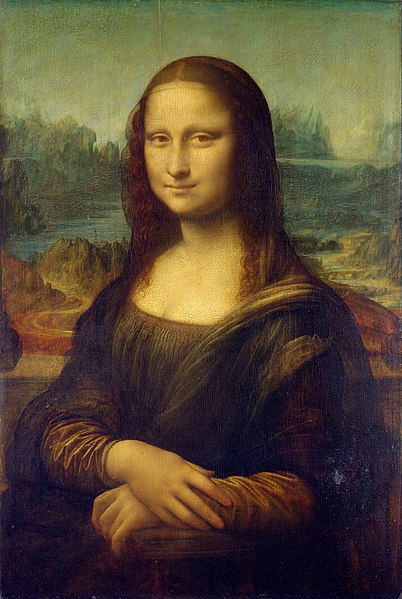
\includegraphics[width=0.45\textwidth]{monalisa}
	\caption[Mona Lisa, again]{It's Mona Lisa again. \blindtext}
	\labfig{normalmonalisa}
\end{figure}

While the format of the caption is managed by \Package{caption}, its 
position is handled by the \Package{floatrow} package. Achieving this 
result has been quite hard, but now I am pretty satisfied. In two-side 
mode, the captions are printed in the correct margin.

Tables can be inserted just as easily as figures, as exemplified by the 
following code:

\begin{lstlisting}[caption={Caption of a listing.}]
\begin{table}
\begin{tabular}{ c c c c }
	\toprule
	col1 & col2 & col3 & col 4 \\
	\midrule
	\multirow{3}{4em}{Multiple row} & cell2 & cell3 & cell4\\ &
	cell5 & cell6 & cell7 \\ &
	cell8 & cell9 & cell10 \\
	\multirow{3}{4em}{Multiple row} & cell2 & cell3 & cell4 \\ &
	cell5 & cell6 & cell7 \\ &
	cell8 & cell9 & cell10 \\
	\bottomrule
\end{tabular}
\end{table}
\end{lstlisting}

which results in the useless \vreftab{useless}.

\begin{table}[ht]
\caption[A useless table]{A useless table.}
\labtab{useless}
\begin{tabular}{ c c c c }
	\toprule
	col1 & col2 & col3 & col 4 \\
	\midrule
	\multirow{3}{4em}{Multiple row} & cell2 & cell3 & cell4\\ &
	cell5 & cell6 & cell7 \\ &
	cell8 & cell9 & cell10 \\
	\multirow{3}{4em}{Multiple row} & cell2 & cell3 & cell4 \\ &
	cell5 & cell6 & cell7 \\ &
	cell8 & cell9 & cell10 \\
	\bottomrule
\end{tabular}
\end{table}

I don't have much else to say, so I will just insert some blind text. 
\blindtext

\section{Margin Figures and Tables}

Marginfigures can be inserted with the environment 
\Environment{marginfigure}. In this case, the whole picture is confined 
to the margin and the caption is below it. \reffig{marginmonalisa} is 
obtained with something like this:

\begin{lstlisting}[caption={Another caption.}]
\begin{marginfigure}
	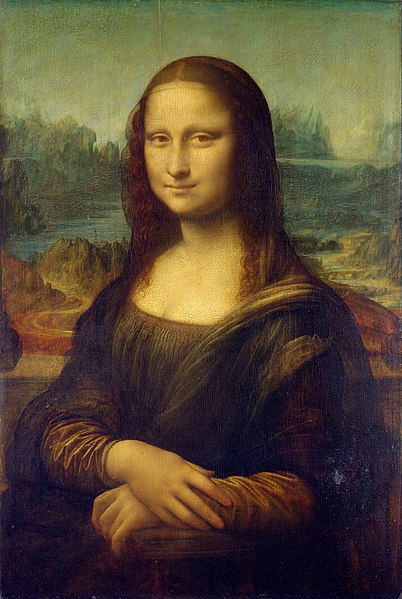
\includegraphics{monalisa}
	\caption[The Mona Lisa]{The Mona Lisa.}
	\labfig{marginmonalisa}
\end{marginfigure}
\end{lstlisting}

There is also the \Environment{margintable} environment, of which 
\reftab{anotheruseless} is an example. Notice how you can place the 
caption above the table by just placing the \Command{caption} command 
before beginning the \Environment{tabular} environment. Usually, figure 
captions are below, while table captions are above. This rule is also 
respected for normal figures and tables: the captions are always on the 
side, but for figure they are aligned to the bottom, while for tables to 
the top.

\begin{margintable}
\caption[Another useless table]{Another useless table.}
\labtab{anotheruseless}
\raggedright
\begin{tabular}{ c c c c }
	\hline
	col1 & col2 & col3 \\
	\hline
	\multirow{3}{4em}{Multiple row} & cell2 & cell3 \\ & cell5 & cell6 
	\\ & cell8 & cell9 \\ \hline
\end{tabular}
\end{margintable}

Marginfigures and tables can be positioned with an optional offset 
command, like so:

\begin{lstlisting}
\begin{marginfigure}[offset]
	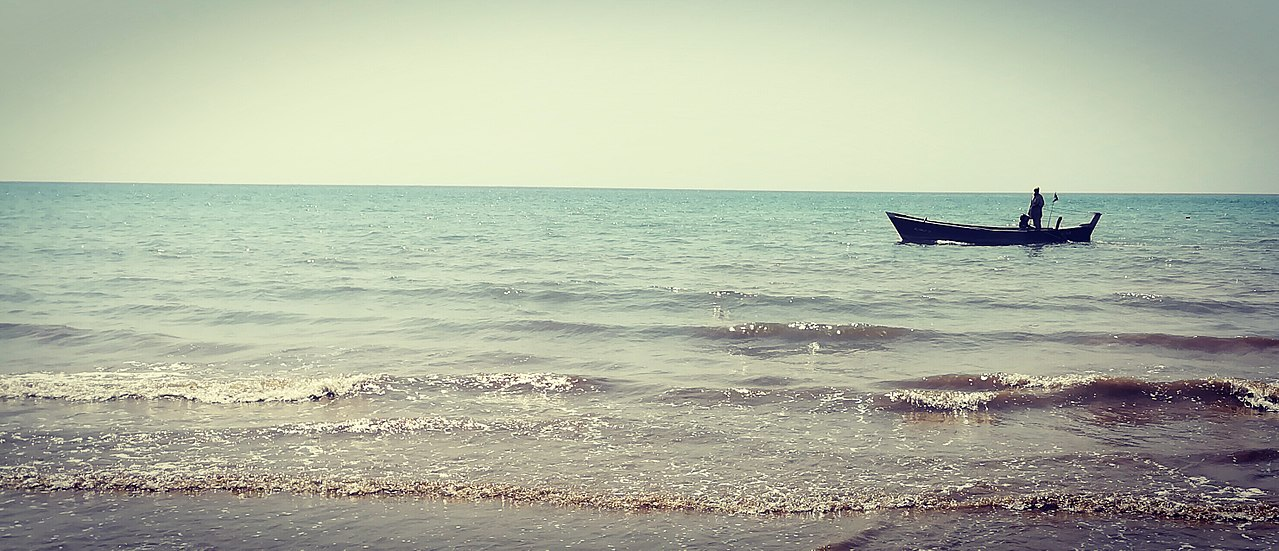
\includegraphics{seaside}
\end{marginfigure}
\end{lstlisting}

Offset ca be either a measure or a multiple of \Command{baselineskip}, 
much like with \Command{sidenote}, \Command{marginnote} and 
\Command{margintoc}.\todo{Improve this part.} If you are wondering how I 
inserted this orange bubble, have a look at the \Package{todo} package.

\section{Wide Figures and Tables}

With the environments \Environment{figure*} and \Environment{table*} you 
can insert figures which span the whole page width. For example, here 
are a wide figure and a wide table.

\begin{figure*}[h!]
	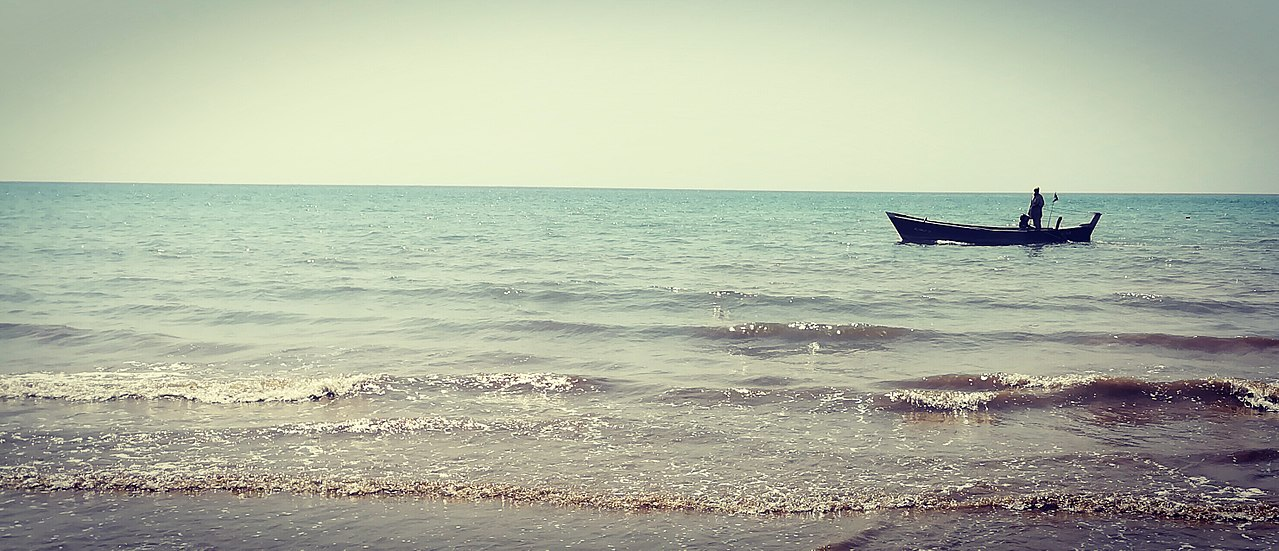
\includegraphics{seaside}
	\caption[A wide seaside]{A wide seaside, and a wide caption.
		Credits: By Bushra Feroz, CC BY-SA 4.0, \url{https://commons.wikimedia.org/w/index.php?curid=68724647}}
\end{figure*}

\begin{table*}[h!]
    \caption{A wide table with invented data about three people living in the UK. Note that wide figures and tables are centered and their caption also extends into the margin.}
    \begin{tabular}{p{2.0cm} p{2.0cm} p{2.0cm} p{2.0cm} p{2.0cm} p{2.0cm} p{1.5cm}}
        \toprule
        Name    & Surname   & Job       & Salary           & Age   & Height    & Country \\
        \midrule
        Alice   & Red       & Writer    & 4.000 \pounds    & 34    & 167 cm     & England \\
        Bob     & White     & Bartender & 2.000 \pounds    & 24    & 180 cm     & Scotland \\
        Drake   & Green     & Scientist & 4.000 \pounds    & 26    & 175 cm     & Wales \\
        \bottomrule
    \end{tabular}
\end{table*}

It is the user's responsibility to adjust the width of the table, if 
necessary, until it is aesthetically pleasing. The previous table was 
obtained with the following code:

\begin{lstlisting}[caption=How to typeset a wide table]
\begin{table*}[h!]
    \caption{A wide table with invented data about three people living in the UK. Note that wide figures and tables are centered and their caption also extends into the margin.}
    \begin{tabular}{p{2.0cm} p{2.0cm} p{2.0cm} p{2.0cm} p{2.0cm} p{2.0cm} p{1.5cm}}
        \toprule
        Name    & Surname   & Job       & Salary           & Age   & Height    & Country \\
        \midrule
        Alice   & Red       & Writer    & 4.000 \pounds    & 34    & 167 cm     & England \\
        Bob     & White     & Bartender & 2.000 \pounds    & 24    & 180 cm     & Scotland \\
        Drake   & Green     & Scientist & 4.000 \pounds    & 26    & 175 cm     & Wales \\
        \bottomrule
    \end{tabular}
\end{table*}
\end{lstlisting}

The \Package{floatrow} package provides the \enquote{H} specifier to 
instruct \LaTeX to position the figure (or table) in precisely the same 
position it occupies in the source code. However, this specifier does 
not work with wide figures or tables: you should use \enquote{h!} 
instead, like so: \lstinline|\begin{figure*}[h!]|.

You may have noticed the full width image at the very beginning of this
chapter: that, however, is set up in an entirely different way, which
you'll read about in \vrefch{layout}.

\Class{kaobook} also supports paginated tables (have a look at the 
\Package{longtable} package). The 
\Environment{longtable}\sidenote{Interestingly, \Environment{longtable}s 
may require up to four rounds of compilation before they are typeset 
correctly.} environment behaves a bit differently from 
\Environment{table}, in that \Environment{longtable} encompasses both 
\Environment{table} and \Environment{tabular}, so that you can write, 
\eg,

\begin{lstlisting}[caption=Example of a longtable]
\begin{longtable}{|l c c|}
    \hline
    One & Two & Three \\
    Left & Center & Center \\
    \hline
    \caption{Caption of the longtable.}
\end{longtable}
\end{lstlisting}

to obtain the following table:
\begin{longtable}{|l c c|}
    \hline
    One & Two & Three \\
    Left & Center & Center \\
    \hline
    \caption{Caption of the longtable.}
\end{longtable}

The caption of a \Environment{longtable} is always positioned below the 
table, and it has the same width as the text (it doesn't extend into the 
margin). However, sometimes you may need a \Environment{longtable} that 
is so wide that it trespass into the margins; in those cases, you may 
want to also increase the width of the caption. To do so, you'll have to 
write two additional commands, one before and one after the 
\Environment{longtable}:

\begin{lstlisting}[caption=Increasing the width of the caption of a \Environment{longtable}.]
\floatsetup[longtable]{margins=centering,LTcapwidth=table} % Add this line before the longtable to increase the caption width
\begin{longtable}{lp{8cm}p{5cm}p{2cm}}
...
\end{longtable}
\floatsetup[longtable]{margins=raggedright,LTcapwidth=\textwidth} % Add this line after the longtable to revert the previous change
\end{lstlisting}

Having seen figures and tables, it is now time to tackle 
hyperreferences.

% \setchapterstyle{kao}
%\setchapterpreamble[u]{\margintoc}
\chapter{References}
\labch{references}

\section{Citations}

\index{citations}
To cite someone \sidecite{Visscher2008,James2013} is very simple: just 
use the \Command{sidecite}\index{\Command{sidecite}} command. It does 
not have an offset argument yet, but it probably will in the future. 
This command supports multiple entries, as you can see, and by default 
it prints the reference on the margin as well as adding it to the 
bibliography at the end of the document. Note that the citations have 
nothing to do with the text,\sidecite{James2013} but they are completely 
random as they only serve the purpose to illustrate the feature.

For this setup I wrote a separate package, \Package{kaobiblio}, which 
you can find in the \Package{styles} directory and include in your main 
tex file. This package accepts all the options that you can pass to 
\Package{biblatex}, and actually it passes them to \Package{biblatex} 
under the hood. Moreover, it also defines some commands, like 
\Command{sidecite}, and environments that can be used within a 
\Class{kao} book.\sidenote[][-.9cm]{For this reason you should always 
use \Package{kaobiblio} instead of \Package{biblatex}, but the syntax 
and the options are exactly the same.}

If you want to use \Package{bibtex} instead of \Package{biblatex},
pass the option \Option{backend=bibtex} to \Package{kaobiblio}.
\Package{kaobiblio} also supports two options that are not shared with
\Package{biblatex}: \Option{addspace} and \Option{linkeverything},
both of which are boolean options, meaning that they can take
either \enquote{true} or \enquote{false} as a value. If you
pass \Option{addspace=true} when loading \Package{kaobiblio},
a space will be automatically added before the citation marks.
If you pass \Option{linkeverything=true}, the author's name in
the authoryear-* and authortitle-* styles will be a hyperlink
like the year.\sidenote{The fact that the author name is not
a hyperlink bothers more than one biblatex user. There are
\href{https://github.com/plk/biblatex/issues/428}{strong arguments}
\emph{against} hyperlinking the author name, but in my personal opinion, 
linking the author's name does not result in any problems in most 
practical cases.}

As you have seen, the \Command{sidecite} command will print a citation 
in the margin. However, this command would be useless without a way to 
customise the format of the citation, so the \Class{kaobook} provides 
also the \Command{formatmargincitation} command. By \enquote{renewing} 
that command, you can choose which items will be printed in the margins. 
The best way to understand how it works is to see the actual definition 
of this command.

\begin{lstlisting}[style=kaolstplain,linewidth=1.5\textwidth]
\newcommand{\formatmargincitation}[1]{%
	\parencite{#1}: \citeauthor*{#1} (\citeyear{#1}), \citetitle{#1}%
}
\end{lstlisting}

Thus, the \Command{formatmargincitation} accepts one parameter, which is 
the citation key, and prints the parencite followed by a colon, then the 
author, then the year (in brackets), and finally the 
title.\sidecite{Battle2014} Now, suppose that you wish the margin 
citation to display the year and the author, followed by the title, and 
finally a fixed arbitrary string; you would add to your document:

\begin{lstlisting}[style=kaolstplain,linewidth=1.5\textwidth]
\renewcommand{\formatmargincitation}[1]{%
	\citeyear{#1}, \citeauthor*{#1}: \citetitle{#1}; very interesting!%
}
\end{lstlisting}

\renewcommand{\formatmargincitation}[1]{%
	\citeyear{#1}, \citeauthor*{#1}: \citetitle{#1}; very interesting!%
}

The above code results in citations that look like the 
following.\sidecite{Zou2005} Of course, changing the format is most 
useful when you also change the default bibliography style. For 
instance, if you want to use the \enquote{philosophy-modern} style for 
your bibliography, you might have something like this in the preamble:

\begin{lstlisting}[style=kaolstplain,linewidth=1.5\textwidth]
\usepackage[style=philosophy-modern]{styles/kaobiblio}
\renewcommand{\formatmargincitation}[1]{%
	\sdcite{#1}%
}
\addbibresource{main.bib}
\end{lstlisting}

\renewcommand{\formatmargincitation}[1]{%
	\parencite{#1}: \citeauthor*{#1} (\citeyear{#1}), \citetitle{#1}%
}

The commands like \Command{citeyear}, \Command{parencite}
and \Command{sdcite} are just examples. A full
reference of the available commands can be found in this
\href{http://tug.ctan.org/info/biblatex-cheatsheet/biblatex-cheatsheet.pdf}{cheatsheet},
under the \enquote{Citations} section.

Finally, to compile a document containing citations, you need to use an 
external tool, which for this class is biber. You need to run the 
following (assuming that your tex file is called main.tex):

\begin{lstlisting}[style=kaolstplain]
$ pdflatex main
$ biber main
$ pdflatex main
\end{lstlisting}

\section{Glossaries and Indices}

\index{glossary}
The \Class{kaobook} class loads the packages \Package{glossaries} and 
\Package{imakeidx}, with which you can add glossaries and indices to 
your book. For instance, I previously defined some glossary entries and 
now I am going to use them, like this: \gls{computer}. 
\Package{glossaries} also allows you to use acronyms, like the 
following: this is the full version, \acrfull{fpsLabel}, and this is the 
short one \acrshort{fpsLabel}. These entries will appear in the glossary 
in the backmatter.

Unless you use \href{https://www.overleaf.com}{Overleaf} or some other 
fancy IDE for \LaTeX, you need to run an external command from your 
terminal in order to compile a document with a glossary. In particular, 
the commands required are:\sidenote{These are the commands you would run 
in a UNIX system, but see also \nrefsec{compiling}; I have no idea about 
how it works in Windows.}

\begin{lstlisting}[style=kaolstplain]
$ pdflatex main
$ makeglossaries main
$ pdflatex main
\end{lstlisting}

Note that you need not run \texttt{makeglossaries} every time you 
compile your document, but only when you change the glossary entries.

\index{index}
To create an index, you need to insert the command 
\lstinline|\index{subject}| whenever you are talking about 
\enquote{subject} in the text. For instance, at the start of this 
paragraph I would write \lstinline|index{index}|, and an entry would be 
added to the Index in the backmatter. Check it out!

\marginnote[2mm]{In theory, you would need to run an external command 
for the index as well, but luckily the package we suggested, 
	\Package{imakeidx}, can compile the index automatically.}

\index{nomenclature}
A nomenclature is just a special kind of index; you can find one at the end of
this book. To insert a nomenclature, we use the package \Package{nomencl} and
add the terms with the command \Command{nomenclature}. We put then a
\Command{printnomenclature} where we want it to appear.

Also with this package we need to run an external command to compile the 
document, otherwise the nomenclature will not appear:

\begin{lstlisting}[style=kaolstplain]
$ pdflatex main
$ makeindex main.nlo -s nomencl.ist -o main.nls
$ pdflatex main
\end{lstlisting}

These packages are all loaded in 
\href{style/packages.sty}{packages.sty}, one of the files that come with 
this class. However, the configuration of the elements is best done in 
the main.tex file, since each book will have different entries and 
styles.

Note that the \Package{nomencl} package caused problems when the 
document was compiled, so, to make a long story short, I had to prevent 
\Package{scrhack} to load the hack-file for \Package{nomencl}. When 
compiling the document on Overleaf, however, this problem seem to 
vanish.

\marginnote[-19mm]{This brief section was by no means a complete 
reference on the subject, therefore you should consult the documentation 
of the above package to gain a full understanding of how they work.}

\section{Hyperreferences}
\labsec{hyprefs}

\index{hyperreferences}
Together with this class we provide a handy package to help you 
referencing the same elements always in the same way, for consistency 
across the book. First, you can label each element with a specific 
command. For instance, should you want to label a chapter, you would put 
\lstinline|\labch{chapter-title}| right after the \Command{chapter} 
directive. This is just a convenience, because \Command{labch} is
actually just an alias to \lstinline|\label{ch:chapter-title}|, so it 
spares you the writing of \enquote{ch:}. We defined similar commands for 
many typically labeled elements, including:

\begin{multicols}{2}
\setlength{\columnseprule}{0pt}
\begin{itemize}
	\item Page: \Command{labpage}
	\item Part: \Command{labpart}
	\item Chapter: \Command{labch}
	\item Section: \Command{labsec}
	\item Figure: \Command{labfig}
	\item Table: \Command{labtab}
	\item Definition: \Command{labdef}
	\item Assumption: \Command{labassum}
	\item Theorem: \Command{labthm}
	\item Proposition: \Command{labprop}
	\item Lemma: \Command{lablemma}
	\item Remark: \Command{labremark}
	\item Example: \Command{labexample}
	\item Exercise: \Command{labexercise}
\end{itemize}
\end{multicols}

Of course, we have similar commands for referencing those elements. 
However, since the style of the reference should depend on the context, 
we provide different commands to reference the same thing. For instance, 
in some occasions you may want to reference the chapter by name, but 
other times you want to reference it only by number. In general, there 
are four reference style, which we call plain, vario, name, and full.

The plain style references only by number. It is accessed, for chapters, 
with \lstinline|\refch{chapter-title}| (for other elements, the syntax 
is analogous). Such a reference results in: \refch{references}.

The vario and name styles rest upon the \Package{varioref} package. 
Their syntax is \lstinline|\vrefch{chapter-title}| and 
\lstinline|\nrefch{chapter-title}|, and they result in: 
\vrefch{references}, for the vario style, and: \nrefch{references}, for 
the name style. As you can see, the page is referenced in 
\Package{varioref} style.

The full style references everything. You can use it with 
\lstinline|\frefch{chapter-title}| and it looks like this: 
\frefch{references}.

Of course, all the other elements have similar commands (\eg for parts 
you would use \lstinline|\vrefpart{part-title}| or something like that). 
However, not all elements implement all the four styles. The commands 
provided should be enough, but if you want to see what is available or 
to add the missing ones, have a look at the 
\href{styles/kaorefs.sty}{attached package}.

In order to have access to all these features, the \Package{kaorefs} 
should be loaded in the preamble of your document. It should be loaded 
last, or at least after \Package{babel} (or \Package{polyglossia}) and 
\Package{plaintheorems} (or \Package{mdftheorems}). Options can be 
passed to it like to any other package; in particular, it is possible to 
specify the language of the captions. For instance, if you specify 
\enquote{italian} as an option, instead of \enquote{Chapter} it will be 
printed \enquote{Capitolo}, the Italian analog. If you know other 
languages, you are welcome to contribute the translations of these 
captions! Feel free to contact the author of the class for further 
details. 

The \Package{kaorefs} package also include \Package{cleveref}, so it is 
possible to use \Command{cref} in addition to all the previously 
described referencing commands.

\section{A Final Note on Compilation}
\labsec{compiling}

Probably the easiest way to compile a latex document is with the 
\Package{latexmk} script, as it can take care of everything, if properly 
configured, from the bibliography to the glossary. The command to issue, 
in general, is:

\begin{lstlisting}
latexmk [latexmk_options] [filename ...]
\end{lstlisting}

\Package{latexmk} can be extensively configured (see
\url{https://mg.readthedocs.io/latexmk.html}). For convenience, I print 
here an example configuration that would cover all the steps described 
above.

\begin{lstlisting}
# By default compile only the file called 'main.tex'
@default_files = ('main.tex');

# Compile the glossary and acronyms list (package 'glossaries')
add_cus_dep( 'acn', 'acr', 0, 'makeglossaries' );
add_cus_dep( 'glo', 'gls', 0, 'makeglossaries' );
$clean_ext .= " acr acn alg glo gls glg";
sub makeglossaries {
   my ($base_name, $path) = fileparse( $_[0] );
   pushd $path;
   my $return = system "makeglossaries", $base_name;
   popd;
   return $return;
}

# Compile the nomenclature (package 'nomencl')
add_cus_dep( 'nlo', 'nls', 0, 'makenlo2nls' );
sub makenlo2nls {
    system( "makeindex -s nomencl.ist -o \"$_[0].nls\" \"$_[0].nlo\"" );
}
\end{lstlisting}

However, if you'd rather not use an external package and want to do 
everything manually, here are some tips.\sidenote{As the author only 
uses Linux and compiles everything from the command line, he doesn't 
know how the compilation works in Windows or Mac. The tips, therefore, 
refer to the usage with Linux from the command line.}

\minisec{Compiling the examples in the kaobook repository}
To compile the examples, and in particular the documentation, that are 
in the \Path{examples} directory of the 
\href{https://github.com/fmarotta/kaobook}{kaobook repository} on 
GitHub, do as follows. \lstinline[language=bash]|cd| into the root 
directory of the repository, and run
\lstinline|pdflatex -output-directory examples/documentation main.tex|. 
With this trick, you can compile the documentation using the class files 
pertaining to the repository (and not, say, those in your texmf tree). 
The \enquote{-output-directory} option works with the other 
\LaTeX-related commands such as biber and makeglossaries.

A note of warning: sometimes \LaTeX\ needs more than one run to get the
correct position of each element; this is true in particular for the
positioning of floating elements like figures, tables, and margin notes.
Occasionally, \LaTeX\ can need up to four re-runs, so If the alignment
of margin elements looks odd, or if they bleed into ther main text, try
runnign pdflatex one more time.


% \pagelayout{wide} % No margins
% \addpart{Design and Additional Features}
% \pagelayout{margin} % Restore margins

% \setchapterimage[6cm]{seaside}
\setchapterpreamble[u]{\margintoc}
\chapter{Page Design}
\labch{layout}

\section{Headings}

So far, in this document I used two different styles for the chapter 
headings: one has the chapter name, a rule and, in the margin, the 
chapter number; the other has an image at the top of the page, and the 
chapter title is printed in a box (like for this chapter). There is one 
additional style, which I used only in the \nrefch{appendix}; there, the chapter title is enclosed in two 
horizontal rules, and the chapter number (or letter, in the case of the 
appendix) is above it.\sidenote{To be honest, I do not think that mixing 
heading styles like this is a wise choice, but in this document I did it 
only to show you how they look.}

Every book is unique, so it makes sense to have different styles from 
which to choose. Actually, it would be awesome if whenever a 
\Class{kao}-user designs a new heading style, he or she added it to the 
three styles already present, so that it will be available for new users 
and new books.

The choice of the style is made simple by the \Command{setchapterstyle} 
command. It accepts one option, the name of the style, which can be: 
\enquote{plain}, \enquote{kao}, \enquote{bar}, or 
\enquote{lines}.\sidenote{Plain is the default \LaTeX\xspace title 
style; the other ones are self explanatory.} If instead you want the 
image style, you have to use the command \Command{setchapterimage}, 
which accepts the path to the image as argument; you can also provide an 
optional parameter in square brackets to specify the height of the 
image. \Command{setchapterimage} automatically sets the chapter style to 
\enquote{bar} for that chapter (and also for subsequent chapters).

Let us make some examples. In this book, I begin a normal chapter with 
the lines:
\begin{lstlisting}
\setchapterstyle{kao}
\setchapterpreamble[u]{\margintoc}
\chapter{Title of the Chapter}
\labch{title}
\end{lstlisting}

In Line 1 I choose the style for the title to be \enquote{kao}. Then, I 
specify that I want the margin toc. The rest is ordinary administration 
in \LaTeX, except that I use my own \Command{labch} to label the 
chapter. Actually, the \Command{setchapterpreamble} is a standard 
\KOMAScript\xspace one, so I invite you to read about it in the KOMA
documentation. Once the chapter style is set, it holds until you change 
it.\sidenote{The \Command{margintoc} has to be specified at every 
chapter. Perhaps in the future this may change; it all depends on how 
this feature will be welcomed by the users, so keep in touch with me if 
you have preferences!} Whenever I want to start a chapter with an image, 
I simply write:

\begin{lstlisting}
\setchapterimage[7cm]{path/to/image.png} % Optionally specify the height
\setchapterpreamble[u]{\margintoc}
\chapter{Catchy Title} % No need to set a chapter style
\labch{catchy}
\end{lstlisting}

If you prefer, you can also specify the style at the beginning of the 
main document, and that style will hold until you change it again.

\section{Headers \& Footers}

Headers and footers in \KOMAScript\xspace are handled by the 
\Package{scrlayer-scrpage} package. There are two basic style: 
\enquote{scrheadings} and \enquote{plain.scrheadings}. The former is 
used for normal pages, whereas the latter is used in title pages (those 
where a new chapter starts, for instance) and, at least in this book, in 
the front matter. At any rate, the style can be changed with the 
\Command{pagestyle} command, \eg 
\lstinline|\pagestyle{plain.scrheadings}|.

In both styles, the footer is completely empty. In plain.scrheadings,
also the header is absent (otherwise it wouldn't be so plain\ldots), but 
in the normal style the design is reminiscent of the \enquote{kao} style
for chapter titles.

\begin{kaobox}[frametitle=To Do]
The \Option{twoside} class option is still unstable and may lead to 
unexpected behaviours. As always, any help will be greatly appreciated.
\end{kaobox}

\section{Table of Contents}

Another important part of a book is the table of contents. By default, 
in \Class{kaobook} there is an entry for everything: list of figures, 
list of tables, bibliographies, and even the table of contents itself. 
Not everybody might like this, so we will provide a description of the 
changes you need to do in order to enable or disable each of these 
entries. In the following \reftab{tocentries}, each item corresponds to 
a possible entry in the \acrshort{tocLabel}, and its description is the 
command you need to provide to have such entry. These commands are 
specified in the attached \href{style/style.sty}{style 
package},\sidenote{In the same file, you can also choose the titles of 
these entries.} so if you don't want the entries, just comment the 
corresponding lines.

Of course, some packages, like those for glossaries and indices, will 
try to add their own entries.\marginnote{In a later section, we will see 
how you can define your own floating environment, and endow it with an 
entry in the \acrshort{tocLabel}.} In such cases, you have to follow the 
instructions specific to that package. Here, since we have talked about 
glossaries and notations in \refch{references}, we will briefly see how
to configure them.

\begin{table}
\footnotesize
\caption{Commands to add a particular entry to the table of contents.}
\labtab{tocentries}
\begin{tabular}{ l l }
	\toprule
	Entry & Command to Activate \\
	\midrule
	Table of Contents & \lstinline|\setuptoc{toc}{totoc}| \\
	List of Figs and Tabs & \lstinline|\PassOptionsToClass{toc=listof}{\@baseclass}| \\
	Bibliography & \lstinline|\PassOptionsToClass{toc=bibliography}{\@baseclass}| \\
	\bottomrule
\end{tabular}
\end{table}

For the \Package{glossaries} package, use the \enquote{toc} option when 
you load it: \lstinline|\usepackage[toc]{glossaries}|. For 
\Package{nomencl}, pass the \enquote{intoc} option at the moment of 
loading the package. Both \Package{glossaries} and \Package{nomencl} are 
loaded in the attached \href{style/packages.sty}{\enquote{packages} 
package}.

Additional configuration of the table of contents can be performed 
through the packages \Package{etoc}, which is loaded because it is 
needed for the margintocs, or the more traditional \Package{tocbase}. 
Read the respective documentations if you want to be able to change the 
default \acrshort{tocLabel} style.\sidenote[][*-1]{(And please, send me 
a copy of what you have done, I'm so curious!)}

\section{Paper Size}

Recent versions of Kaobook support paper sizes different from the
default A4. It is possible to pass the name of the paper as an option
to the class, as we are accustomed for any other \LaTeX\ class. For
example, the class option \Option{b5paper} would set the paper size
to the B5 format.

We also support the paper sizes specified in
\href{https://www.bod.de/hilfe/hilfe-und-service.html?cmd=SINGLE\&entryID=2494\_GER\_WSS\&eo=2\&title=welche-buchformate-gibt-es}{this
web page} and some additional sizes requested by the users, with the 
option names specified in \reftab{papersizes}.

\begin{margintable}[*-6]
	\caption{Some non-standard paper sizes supported by kaobook.}
	\labtab{papersizes}
	\begin{tabular}{ll}
		\toprule
		Dimension & Option name \\
		\midrule
		12.0cm x 19.0cm & smallpocketpaper \\
		13.5cm x 21.5cm & pocketpaper \\
		14.8cm x 21.0cm & a5paper \\
		15.5cm x 22.0cm & juvenilepaper \\
		17.0cm x 17.0cm & smallphotopaper \\
		21.0cm x 15.0cm & appendixpaper \\
		17.0cm x 22.0cm & cookpaper \\
		19.0cm x 27.0cm & illustratedpaper \\
		17.0cm x 17.0cm & photopaper \\
		16.0cm x 24.0cm & f24paper \\
		%21.0cm x 29.7cm & a4paper \\
		\bottomrule
	\end{tabular}
\end{margintable}

For instance, to use the \enquote{smallpocketpaper} add the correct 
description at the beginning of the documentclass instruction:
\begin{lstlisting}
\documentclass[
		smallpocketpaper,
		fontsize=10pt,
		twoside=false,
		%open=any,
		secnumdepth=1,
]{kaobook}
\end{lstlisting}

\section{Page Layout}

Besides the page style, you can also change the width of the content of 
a page. This is particularly useful for pages dedicated to part titles, 
where having the 1.5-column layout might be a little awkward, or for 
pages where you only put figures, where it is important to exploit all 
the available space.

In practice, there are two layouts: \enquote{wide} and \enquote{margin}. 
The former suppresses the margins and allocates the full page for 
contents, while the latter is the layout used in most of the pages of 
this book, including this one. The wide layout is also used 
automatically in the front and back matters.

\marginnote{Sometimes it is desirable to increase the width for just one 
or a few paragraphs; the \Environment{widepar} environment does that: 
wrap your paragraphs in this environment, and they will occupy the full 
width of the page.}

To change page layout, use the \Command{pagelayout} command. For 
example, when I start a new part, I write:

\begin{lstlisting}
\pagelayout{wide}
\addpart{Title of the New Part}
\pagelayout{margin}
\end{lstlisting}

Beyond these two basic layouts, it is also possible to finely tune the 
page layout by redefining the \Command{marginlayout} command. This 
command is called internally by the higher-level \Command{pagelayout}, 
and it is responsible for setting the width of the margins and of the 
text. The default definition is:

\begin{lstlisting}
\newcommand{\marginlayout}{%
	\newgeometry{
		top=27.4mm,				% height of the top margin
		bottom=27.4mm,			% height of the bottom margin
		inner=24.8mm,			% width of the inner margin
		textwidth=107mm,		% width of the text
		marginparsep=8.2mm,		% width between text and margin
		marginparwidth=49.4mm,	% width of the margin
	}%
}
\end{lstlisting}

so if you want to, say, decrease the width of the margin while 
increasing the width of the text, you could write in the preamble of 
your document something like:

\begin{lstlisting}
\renewcommand{\marginlayout}{%
	\newgeometry{
		top=27.4mm,				% height of the top margin
		bottom=27.4mm,			% height of the bottom margin
		inner=24.8mm,			% width of the inner margin
		textwidth=117mm,		% width of the text
		marginparsep=8.2mm,		% width between text and margin
		marginparwidth=39.4mm,	% width of the margin
	}%
}
\end{lstlisting}

where the text width has been increased by 10mm and the margin width has 
been decreased by 10mm.

\section{Numbers \& Counters}

In this short section we shall see how dispositions, sidenotes and 
figures are numbered in the \Class{kaobook} class.

By default, dispositions are numbered up to the section in \Class{kaobook}
and up to the subsection in \Class{kaohandt}. This can be changed by
passing the option \Option{secnumdepth} to\Class{kaobook} or
\Class{kaohandt} (e.g. 1 corresponds to section and 2 corresponds to
subsections).

The sidenotes counter is the same across all the document, but if you 
want it to reset at each chapter, just uncomment the line

\begin{lstlisting}[style=kaolstplain]
\counterwithin*{sidenote}{chapter}
\end{lstlisting}

in the \Package{styles/style.sty} package provided by this class.

Figure and Table numbering is also per-chapter; to change that, use 
something like:

\begin{lstlisting}[style=kaolstplain]
\renewcommand{\thefigure}{\arabic{section}.\arabic{figure}}
\end{lstlisting}

\section{White Space}

One of the things that I find most hard in \LaTeX\xspace is to finely 
tune the white space around objects. There are not fixed rules, each 
object needs its own adjustment. Here we shall see how some spaces are 
defined at the moment in this class.\marginnote{Attention! This section 
may be incomplete.}

\textbf{Space around sidenotes and citations marks}

There should be no space before or after sidenotes and citation marks, 
like so:

sidenote\sidenote{This paragraph can be used to diagnose any problems:
if you see whitespace around sidenotes or citation marks, probably
a \% sign is missing somewhere in the definitions of the class
macros.}sidenote\newline
citation\cite{James2013}citation

\textbf{Space around figures and tables}

\begin{lstlisting}[style=kaolstplain]
\renewcommand\FBaskip{.4\topskip}
\renewcommand\FBbskip{\FBaskip}
\end{lstlisting}

\textbf{Space around captions}

\begin{lstlisting}[style=kaolstplain]
\captionsetup{
	aboveskip=6pt,
	belowskip=6pt
}
\end{lstlisting}

\textbf{Space around displays (\eg equations)}

\begin{lstlisting}[style=kaolstplain]
\setlength\abovedisplayskip{6pt plus 2pt minus 4pt}
\setlength\belowdisplayskip{6pt plus 2pt minus 4pt}
\abovedisplayskip 10\p@ \@plus2\p@ \@minus5\p@
\abovedisplayshortskip \z@ \@plus3\p@
\belowdisplayskip \abovedisplayskip
\belowdisplayshortskip 6\p@ \@plus3\p@ \@minus3\p@
\end{lstlisting}

% \setchapterstyle{kao}
\setchapterpreamble[u]{\margintoc}
\chapter{Mathematics and Boxes}
\labch{mathematics}

\section{Theorems}

Despite most people complain at the sight of a book full of equations, 
mathematics is an important part of many books. Here, we shall 
illustrate some of the possibilities. We believe that theorems, 
definitions, remarks and examples should be emphasised with a shaded 
background; however, the colour should not be to heavy on the eyes, so 
we have chosen a sort of light yellow.\sidenote{The boxes are all of the 
same colour here, because we did not want our document to look like 
\href{https://en.wikipedia.org/wiki/Harlequin}{Harlequin}.}

\begin{definition}
\labdef{openset}
Let $(X, d)$ be a metric space. A subset $U \subset X$ is an open set 
if, for any $x \in U$ there exists $r > 0$ such that $B(x, r) \subset 
U$. We call the topology associated to d the set $\tau\textsubscript{d}$ 
of all the open subsets of $(X, d).$
\end{definition}

\refdef{openset} is very important. I am not joking, but I have inserted 
this phrase only to show how to reference definitions. The following 
statement is repeated over and over in different environments.

\begin{theorem}
A finite intersection of open sets of (X, d) is an open set of (X, d), 
i.e $\tau\textsubscript{d}$ is closed under finite intersections. Any 
union of open sets of (X, d) is an open set of (X, d).
\end{theorem}

\begin{proposition}
A finite intersection of open sets of (X, d) is an open set of (X, d), 
i.e $\tau\textsubscript{d}$ is closed under finite intersections. Any 
union of open sets of (X, d) is an open set of (X, d).
\end{proposition}

\marginnote{You can even insert footnotes inside the theorem 
environments; they will be displayed at the bottom of the box.}

\begin{lemma}
A finite intersection\footnote{I'm a footnote} of open sets of (X, d) is 
an open set of (X, d), i.e $\tau\textsubscript{d}$ is closed under 
finite intersections. Any union of open sets of (X, d) is an open set of 
(X, d).
\end{lemma}

You can safely ignore the content of the theorems\ldots I assume that if 
you are interested in having theorems in your book, you already know 
something about the classical way to add them. These example should just 
showcase all the things you can do within this class.

\begin{corollary}[Finite Intersection, Countable Union]
A finite intersection of open sets of (X, d) is an open set of (X, d), 
i.e $\tau\textsubscript{d}$ is closed under finite intersections. Any 
union of open sets of (X, d) is an open set of (X, d).
\end{corollary}

\begin{proof}
The proof is left to the reader as a trivial exercise. Hint: \blindtext
\end{proof}

\begin{definition}
Let $(X, d)$ be a metric space. A subset $U \subset X$ is an open set 
if, for any $x \in U$ there exists $r > 0$ such that $B(x, r) \subset 
U$. We call the topology associated to d the set $\tau\textsubscript{d}$ 
of all the open subsets of $(X, d).$
\end{definition}

\marginnote{
	Here is a random equation, just because we can:
	\begin{equation*}
  x = a_0 + \cfrac{1}{a_1
          + \cfrac{1}{a_2
          + \cfrac{1}{a_3 + \cfrac{1}{a_4} } } }
	\end{equation*}
}

\begin{example}
Let $(X, d)$ be a metric space. A subset $U \subset X$ is an open set 
if, for any $x \in U$ there exists $r > 0$ such that $B(x, r) \subset 
U$. We call the topology associated to d the set $\tau\textsubscript{d}$ 
of all the open subsets of $(X, d).$
\end{example}

\begin{remark}
Let $(X, d)$ be a metric space. A subset $U \subset X$ is an open set 
if, for any $x \in U$ there exists $r > 0$ such that $B(x, r) \subset 
U$. We call the topology associated to d the set $\tau\textsubscript{d}$ 
of all the open subsets of $(X, d).$
\end{remark}

As you may have noticed, definitions, example and remarks have 
independent counters; theorems, propositions, lemmas and corollaries 
share the same counter.

\begin{remark}
Here is how an integral looks like inline: $\int_{a}^{b} x^2 dx$, and 
here is the same integral displayed in its own paragraph:
\[\int_{a}^{b} x^2 dx\]
\end{remark}

There is also an environment for exercises.

\begin{exercise}
Prove (or disprove) the Riemann hypothesis.
\end{exercise}

We provide one package for the theorem styles: 
\href{kaotheorems.sty}{kaotheorems.sty}, to which you can pass the 
\Option{framed} option you do want coloured boxes around theorems, like 
in this document.\sidenote{The styles without \Option{framed} are not 
showed, but actually the only difference is that they don't have the 
yellow boxes.} You may want to edit this files according to your taste 
and the general style of the book. However, there is an option to 
customise the background colour of the boxes if you use the 
\Option{framed} option: when you load this package, you can pass it the 
\Option{background=mycolour} option (replace \enquote{mycolour} with the 
actual colour, for instance, \enquote{red!35!white}). This will change 
the colour of all the boxes, but it is also possible to override the 
default colour only for some elements. For instance, the 
\Option{propositionbackground=mycolour} option will change the colour 
for propositions only. There are similar options for theorem, 
definition, lemma, corollary, remark, and example.

\section[Boxes \& Environments]{Boxes \& Custom Environments
\sidenote[][*1.8]{Notice that in the table of contents and in the 
	header, the name of this section is \enquote{Boxes \& Environments}; 
	we achieved this with the optional argument of the \texttt{section} 
	command.}}

Say you want to insert a special section, an optional content or just 
something you want to emphasise. We think that nothing works better than 
a box in these cases. We used \Package{mdframed} to construct the ones 
shown below. You can create and modify such environments by editing the 
provided file \href{style/environments.sty}{environments.sty}.

\begin{kaobox}[frametitle=Title of the box]
\blindtext
\end{kaobox}

If you set up a counter, you can even create your own numbered 
environment.

\begin{kaocounter}
	\blindtext
\end{kaocounter}

\section{Experiments}

It is possible to wrap marginnotes inside boxes, too. Audacious readers 
are encouraged to try their own experiments and let me know the 
outcomes.

\marginnote[-2.2cm]{
	\begin{kaobox}[frametitle=title of margin note]
		Margin note inside a kaobox.\\
		(Actually, kaobox inside a marginnote!)
	\end{kaobox}
}

I believe that many other special things are possible with the 
\Class{kaobook} class. During its development, I struggled to keep it as 
flexible as possible, so that new features could be added without too 
great an effort. Therefore, I hope that you can find the optimal way to 
express yourselves in writing a book, report or thesis with this class, 
and I am eager to see the outcomes of any experiment that you may try.

%\begin{margintable}
	%\captionsetup{type=table,position=above}
	%\begin{kaobox}
		%\caption{caption}
		%\begin{tabular}{ |c|c|c|c| }
			%\hline
			%col1 & col2 & col3 \\
			%\hline
			%\multirow{3}{4em}{Multiple row} & cell2 & cell3 \\ & cell5 
			%%& cell6 \\ 
			%& cell8 & cell9 \\
			%\hline
		%\end{tabular}
	%\end{kaobox}
%\end{margintable}


\appendix % From here onwards, chapters are numbered with letters, as is the appendix convention

\pagelayout{wide} % No margins
\addpart{Appendix}
\pagelayout{margin} % Restore margins
\setchapterstyle{lines}
% ===========================================
% SYLLABUS
% Written by: Braidan Duffy
%
% Date: 05/22/2022
% Last Revision: 05/25/2022
% ============================================

\pagelayout{wide} % Remove margins
\chapter{Syllabus} 
\labch{syllabus}

\section*{Course Description} \labsec{course_desc}
This course is intended to give students exposure to practical electronic design and grant them additional programming experience. 
All of this will be accomplished through the lens of developing an instrumentation package that can be deployed as a project and capture/record data. 
Students will use basic Arduino learning kits to cultivate their interests. 
Graduate students taking the course will be required to follow more industry-related programming practices for the Arduino programming, will be held to a higher product quality standard, and will be required to develop a more advanced instrumentation package than the undergraduates. 
Course lectures will be supplemented by weekly (or as weekly as possible) demonstrations using real measurement equipment used by the Ocean Engineering department.

    \subsection*{Meeting Times}
        \subsubsection*{Lectures}
        Monday, Wednesday, Friday; 16:00-16:50 (0h50min)\\
        Fall 2022, August 22 - December 9\\
        Room TBD

        \subsubsection*{Office Hours}
        Monday, Wednesday, Friday; 13:00-15:00\\
        Or, by appointment (preferred)\\
        Link 155 or Frueauff 100

    \subsection*{Objectives \& Outcomes}
    The goal of this course is the provide a basic instruction on practical electrical engineering and computer programming through the lens of instrumentation design. 
    After introducing and refreshing basic concepts like electrical components, digital electronics, and C++ basics, students will be taught how industry professionals make real-world measurements using various instruments. At the end of the course, students will be able to:
    \begin{enumerate}
        \item Understand how various measurement devices capture, record, and transmit information to researchers and engineers
        \item Have a fundamental knowledge of programming Arduino-based microcontrollers
        \item Have a fundamental knowledge of Printed Circuit Board design, manufacture, and assembly
        \item Apply the fundamental concepts learned in lecture and through demonstrations on a practical Individual Course Project.
    \end{enumerate}

    \subsection*{Target Audience \& Prerequisites}
    On the undergraduate side, this course is intended for students who do not have a basic familiarity with basic electronics and programming with Arduino. 
    The ELEGOO Arduino Starter Kit recommended for this class has supplementary information that will assist students in understanding exactly what is occurring with various projects. 
    Students are strongly encouraged to delve deeper into the topics covered in class and pursue a challenging Individual Course Project. 
    Individuals with a strong drive to learn independently will benefit greatly during this course.

    On the graduate side, this course is designed for students who have a basic knowledge of electronics and programming with Arduino or C++. 
    Embedded design experience is also desired as it will be most beneficial during the Individual Course Project. 
    While the ELEGOO Arduino Starter Kit will give the basics, graduate students will be expected to expand upon the projects covered in the kit and use more sophisticated programming techniques. 
    The Individual Course Project will also need to be well considered and adequately demonstrate the student's knowledge and motivation to learn outside the classroom.

    \subsection*{Course Resources}
    The course material will be regularly updated on Canvas and \href{https://github.com/Legohead259/OCE4531-Material} {GitHub}. The GitHub repository will have all of the supplementary and study material required by students. The Canvas page may also contain these files, but GitHub will be the most up to date.
    
    Students will be \emph{required} to purchase their own Arduino learning kit for this course. They can be easily found on Amazon.
    
    \begin{enumerate}
        \item \href{https://www.amazon.com/ELEGOO-Project-Tutorial-Controller-Projects/dp/B01D8KOZF4}
        {UNO R3 Super Starter Kit - \$34}
        \item \href{https://www.amazon.com/EL-KIT-001-Project-Complete-Starter-Tutorial/dp/B01CZTLHGE} 
        {UNO R3 Complete Starter Kit - \$60}
        \item \href{https://www.amazon.com/EL-KIT-008-Project-Complete-Ultimate-TUTORIAL/dp/B01EWNUUUA}
        {Mega R3 Complete Ultimate Starter Kit - \$55}
    \end{enumerate}

    Graduate students will also be required to order a Raspberry Pi - or equivalent Single Board Computer (SBC), for this course. 
    It is strongly recommended to purchase a Raspberry Pi 400 Full Computer Kit (\href{https://www.adafruit.com/product/4796}{Adafruit}) with an accompanying T-Cobbler GPIO Breakout (\href{https://www.adafruit.com/product/2028}{Adafruit}).
    
    Due to the recent chip shortage, Raspberry Pis may be hard to find or prohibitively expensive. If students are unable to acquire their own Raspberry Pis or similar SBCs, they may ask for a loaner unit from the instructor. \textbf{Please note that if the loaner unit is \emph{not} returned by the end of the semester, the student will be given an ``Incomplete'' grade until the instructor has been given the device.}

\pagebreak

\section*{Grading Policies}
This course covers several student performance metrics: (i) assignments, (ii) participation, (iii) midterm exam, and (iv) an Individual Course Project. The weighting for this metrics is below:

\begin{table*}[ht!]
    \begin{tabular}{c | c}
        \toprule
        Metric                      & Weight \\

        \midrule
        Assignments                 & 20\% \\
        Participation               & 10\% \\
        Midterm Exam                & 30\% \\
        Individual Course Project   & 40\% \\

        \bottomrule
    \end{tabular}
\end{table*}

Students will be assigned the following letter grade and GPA quality points based on their weighted sum assignment scores according to:

\begin{table*}[h!]
    \begin{tabular}{c | c | c}
        \toprule
        Score & Letter Grade & Quality Points \\
        
        \midrule
        90-100              & A     & 4 \\
        80-89               & B     & 3 \\
        70-79               & C     & 2 \\
        60-69\footnotemark  & D     & 1 \\
        <60                 & F     & 0 \\

        \bottomrule
    \end{tabular}
\end{table*}
\footnotetext{Undergraduate students only. \textbf{Graduate students will fail below a 70.}}

\section*{Course Schedule}
\begin{table*}[h!]
    \begin{tabular}{ c | c | c | c }
        \toprule
        Week & Monday & Wednesday & Friday \\

        \midrule
        1   & Syllabus, setup       & Binary and boolean logic          & Project discussion    \\
        2   & Digital logic         & Digital logic                     & YSI Castaway demo     \\    
        3   & \textbf{NO CLASS}     & Multiplexers, registers, states   & HOBO meter demo       \\
        4   & ADC Conversion        & Communication methods             & Survey gear demo      \\
        5   & Electrical comps      & Simple circuit debugging          & Launchsonde demo      \\
        6   & Intro to Fusion 360   & ECAD-Schematics                   & Lowell/Thetis demo    \\
        7   & ECAD-Schematics       & ECAD-PCB basics                   & Sidescan SONAR demo   \\
        8   & \textbf{NO CLASS}     & Inertial Measurement Units        & Midterm exam          \\
        9   & Sensor Fusion         & AHRS design                       & CODAR system demo     \\
        10  & Distance sensors      & Environmental sensors             & Soldering workshop    \\
        11  & Analog filtering      & Digital filtering                 & Remote sensing demo   \\
        12  & Gerber gen. and order & PCB manufacture techniques        & \textbf{NO CLASS}     \\
        13  & PCB assembly (hand)   & PCB assembly (PnP)                & Robotics demo         \\
        14  & Buffer day            & \textbf{NO CLASS}                 & \textbf{NO CLASS}     \\
        15  & Data transmission     & Power considerations              & Work day              \\
        16  & ICP Presentations     & ICP Presentations                 & ICP Presentations     \\

        \bottomrule
    \end{tabular}
\end{table*}

\pagebreak

\section*{Assignment Schedule} \labsec{assignment_sch}
\begin{table*}[h!]
    \begin{tabular}{ l | c }
        \toprule
        Assignment & Due Date \\

        \midrule
        Get Arduino Kit, Raspberry Pi\footnotemark                  & August 26     \\
        Project 1: RGB LED                                          & August 29     \\
        Project 2: Digital inputs and interrupts                    & September 7   \\
        Project 3: 7-Segment Counter, ICP: Proposal\footnotemark[2] & September 19  \\
        Project 4: Sensor module and display                        & October 14     \\
        Midterm Exam                                                & October 14    \\
        ICP: Schematic                                              & October 24    \\
        ICP: PCB design                                             & November 11   \\
        ICP: Assembled PCB                                          & November 28   \\
        ICP: Final presentation                                     & December 5    \\
        ICP: Final report                                           & December 12   \\

        \bottomrule
    \end{tabular}
\end{table*}
\footnotetext[2]{Graduate students only}

\section*{Other Important Dates}

\begin{table*}[h!]
    \begin{tabular}{ l | c }
        \toprule
        Event & Date \\

        \midrule
        Last day to drop without a "W"  & August 31 \\
        Last day to drop with a "W"     & October 31 \\

        \bottomrule
    \end{tabular}
\end{table*}

\section*{Course Policies} \labsec{course_policies}
    \subsection*{Online Course Management}
    This course will be published in the online learning tool, \href{instructure.fit.edu}{Canvas}, and will be made readily available to all students. 
    Canvas provides an online cross-platform solution for students and instructors to engage and will handle all of the assignment submissions and \emph{preliminary} grades for students.
    Assignments will be issued and submitted through the Canvas platform and students will be expected to submit the required documents by the due date and time listed on the assignment submission box.
    If, for whatever reason, assignments are unable to be turned in through Canvas, they must be emailed to the instructor and timestamped by the date and time established.
    
    Grades will also be posted on Canvas for students to track their progress in status in the course.
    However, there is no guarantee that the posted grade in Canvas will represent the final course grade submitted to the registrar, nor may it be up-to-date if grade corrections are necessary.
    In the event a student is not satisfied by their grade posted in Canvas, they are more than welcome to schedule a \emph{face-to-face} meeting with the instructor to discuss.
    Emailed requests to change grades may be considered but it will be more effective to meet with the instructor in-person to ensure the change is made properly.

    Canvas will also have a "Files" section where students can find relevant course resources and documents to aid in their studies.
    Students may request certain documents be uploaded to Canvas to share with their classmates and they may download all files freely if they wish to have their own local copies.
    The Canvas may be periodically updated to reflect changes or addendums to course content, but it may not necessarily reflect the most up-to-date information.
    For the most updated course material, please consult the class \href{https://github.com/OCE4531-Materials}{GitHub Repository}. \emph{You may be surprised what you find in there...}

    \subsection*{Weekly Projects}
    For the first couple of weeks of the course, students will be expected to put their Arduino starter kits to use with various projects.
    These are intended to slowly ramp up in complexity and give students a glimpse of what practical electronics and programming looks like.
    Projects will be due by 23:59 Eastern Time on the day specified in the \hyperref[sec:assignment_sch]{Assignment Schedule} section.
    
    \paragraph*{Late Policy} Submissions for assignments will be accepted up to the date of the students ICP presentation.
    However, for every day (24 hours) after the deadline, starting the minute after the deadline passes, 10 points will be deducted from the assignment down to an absolute maximum of 50\%.


    \subsection*{Individual Course Project}
    The Individual Course Project (ICP) is designed to encompass all of the elements taught throughout the course into a single package.
    Undergraduate students will be tasked with taking one of the Arduino projects available in their starter kits and converting it to an Arduino-compatible shield.
    Essentially, taking the circuit they already made on a breadboard, drawing the schematic in an ECAD software like Fusion 360, routing the PCB in the same software, and order and assembling the final PCB. 
    Students will be tasked with writing up their ICP in a comprehensive report and giving a quick final presentation at the end of the semester.

    \paragraph*{Financial Policy} Students will be required to purchase their PCBs and any additional components for their ICP not already available to them in their Arduino kits or by the Underwater Technology Lab. 
    Currently, each student is expected to pay around \$5 for the PCB order and most undergraduate students should be using components already present in their Arduino kits. 
    The final amount each student will have to pay for their PCB will be determined at the time of ordering by the instructor.
    
    Sponsorship by the UTL may be requested and may be granted on a case-by-case basis. Students with ICPs that prove useful to the lab's operation may have their fees waived depending on several external factors.
    This will be determined by the time of ordering.
    Students wishing to be sponsored should contact the instructor ASAP for details.

    \paragraph*{Failure Policy} \emph{FAILURE IS AN OPTION.} It is well-understood that students may have a non-functional ICP at the end of the semester. \textbf{That is okay!}
    The university environment is about learning and especially learning while failing.
    Therefore, students who do not have a functional PCB have two options for recourse:
    \begin{enumerate}
        \item they may explain, in copious detail, what the failure on the PCB was and how it would be addressed in the next revision, were it to be manufactured. 
        \item they will have until December 12 to submit a fixed PCB that is working, but may have "bodges" or other modifications
    \end{enumerate}
    If students elect for Option 1, they will receive penalty points on their ICP. These points will be subjectively detracted according to the instructor. As a general guideline, \emph{the simpler the mistake, the harsher the penalty will be}. 
    For instance, a missing connection in the schematic or trace on the PCB will have more points deducted than two components not talking due to EMI or other nuanced electrical engineering problem.
    \emph{Attention to detail is important!}

    \paragraph*{Late Policy} Late submissions on any part of the ICP will not be tolerated. For every 24 hours after the minute an ICP-related assignment is due, 10\% will be deducted from the \textbf{overall} ICP grade.
    Simply put, if four ICP-related assignments are turned in a minute late, then the student will be limited to a maximum grade of a C in the course.
    
    Additionally, students who do not submit a PCB gerber package by the order deadline (November 11) may end up forfeiting their potential grades.
    This deadline is in place to ensure ample time for PCB assembly and testing and all orders will be placed at the same time.
    If a student does not submit the PCB gerber package by the deadline, the onus and financial responsibility will be on them to order the PCBs in a timely manner such that they can still assemble and test their ICP.

    \subsection*{For Students with Handicaps and/or Disabilities}
    Students with handicaps and/or disabilities will be given special considerations depending on their condition and Florida Tech policy. Please meet with the instructor privately to discuss any concerns or arrangements. 

    \subsection*{Academic Dishonesty Policy}
    Students who are caught cheating or plagiarizing will be given an audience with the instructor to discuss the situation. 
    Some cases are simple mistakes or coincidences with no ill-intent and can be rectified with a penalty to the assignment grade.
    Severe cases of rampant cheating or plagiarism \emph{with} ill-intent or gross negligence will be referred to the Dean of Students in accordance with academic policy present in the Florida Tech handbook.
    Students who are referred to the Dean of Students may forfeit their overall grades for the course and may face academic probation, suspension, or expulsion from Florida Tech - as the Dean determines.
    
    Academic Dishonesty incidents will not be considered until the assignment is officially submitted. 
    Therefore, students are strongly encouraged to meet with the instructor with questions about if a portion of their assignment could be considered academically dishonest.

    \subsection*{Title IX}
    Title IX of the Educational Amendments Act of 1972 is the federal law prohibiting discrimination based on sex under any education program and/or activity operated by an institution receiving and/or benefiting from federal financial assistance. Behaviors that can be considered “sexual discrimination” include sexual assault, sexual harassment, stalking, relationship abuse (dating violence and domestic violence), sexual misconduct, and gender discrimination. You are encouraged to report these behaviors. The instructor and all other faculty and staff are \emph{legally required} to report an incidents they know about, directly or otherwise, to institute administration.

    \paragraph*{Reporting} Florida Tech can better support students in trouble if we know about what is happening.  Reporting also helps us to identify patterns that might arise - for example, if more than one complainant reports having been assaulted or harassed by the same individual. We can only help if you let us.

    \subsection*{Regarding Unusual or Extraneous Circumstances}
    \emph{``If anything can go wrong, it will'' - Murphy's Law}

    It is well-understood that incidents will occur in this fickle thing we call life.
    Students and instructors alike are human and we cannot predict what will happen in the next five minutes let alone the next few days.
    In the event of something unexpected or unusual, please contact the instructor ASAP.
    Each case will be considered for its severity, impact on student well-being, and impact to the student's education.
    Some unforeseen circumstances may warrant an extension to an assignment deadline, a reschedule of a test, or other remedies depending on its severity.
    
    Conversely, the instructor may have incidents where class may need to be cancelled or an assignment delayed. The instructor reserves the right to maneuver the class as they see fit, but it would not be possible without the participation of the students.
    If the instructor is late to class, please allow for up to 15 minutes before departing.
    If the instructor needs to cancel a class, there will be an announcement made through the Canvas page, ideally, well ahead of the class start time.
    Additionally, the instructor may elect to hold class in a remote session through Zoom, should that be a necessary option.
    
    Students, please try to be flexible and understanding, and the instructors will do the same.

\pagelayout{margin} % Restore margins
% ===========================================
% Project 1: RGB LED Cycler
% Written by: Braidan Duffy
%
% Date: 05/22/2022
% Last Revision: 05/25/2022
% ============================================

\chapter{Project 1: RGB LED Cycler}
\labch{p1_rgb_led}

\section*{Overview}
In this project, you will use the RGB LED within your Arduino kit to learn the basics of digital inputs, PWM output, switch-case statements, functions, and various loops.
The goal of this project will be to activate different modes on the RGB LED using a button to cycle through them and a switch-case statement to execute the appropriate functions.
Since this is a beginning project, there is some psuedocode below to give you an idea of how the code should be structured.
It will be up to you to determine what specific functions you want your LED to perform.

\section*{Requirements}
For this project, you must successfully hook up a button, an RGB LED, and any supporting passive components your Arduino and breadboard.
\marginnote{\textbf{Reminder:} The LED \emph{must} be connected to the Arduino pins with resistors in series in order to protect the diodes. Please consult your Arduino kit manual for specific resistor values}
You must also have at least three different functions that your LED performs - one of which must include loop. A great example would be the rainbow loop found in Example \ref{} or the breathe example found in Example \ref{} \todo{make these examples and put it in the book}

\section*{Submission}
You will be required to submit the following on Canvas:
\begin{outline}
    \1 a video of the project working with narration of what is occurring
    \1 a well-organized and documented schematic of the project setup
    \1 the source code file
\end{outline}
Please package all of these items into a compressed (zipped) folder and upload them to Canvas.

\section*{Grading}
You will be graded along the following criteria:

\begin{table}
    \begin{tabular}{ l | c }
        \toprule
        Criterion & Points \\

        \midrule
        Efficacy & 60 \\
        Schematic neatness & 20 \\
        Code neatness & 20 \\
        Mystery extra credit & 10 \\

        \bottomrule
    \end{tabular}
\end{table}

\section*{Extra Credit}
If you are willing to dig in a little bit more, this project has a couple of opportunities to earn extra credit points at the discretion of the instructor.
Implementing something unique with the RGB LED or the button input will warrant the extra credit points.
\marginnote{\textbf{Hint:} Research the problem with button inputs}
If you want to try and get the extra credit points, please let the instructor know in the submission and detail why you believe you earn the points.

\section*{Psuedocode}

\begin{lstlisting}[linewidth=1.5\textwidth]
Program: RGB LED Cycler

Define an input button pin as some Arduino pin
Define the red LED pin as some Arduino pin
Define the green LED pin as some Arduino pin
Define the blue LED pin as some Arduino pin
Define the number of LED functions as the number of modes you want

Initialize the current LED mode as 0

Function: Setup
    Initialize Serial communication for debugging
    Initialize input pins
    Initialize output pins

Function: Loop
    Check for button pressed
    If button is pressed then
        If the current LED mode is the last LED mode
            Reset the current LED mode to the first one
        Else
            Increment the LED mode by 1
    Switch the current LED mode
        Case the current LED mode is set to 0
            Execute first LED function
        Case the current LED mode is set to 1
            Execute second LED function
        Case the current LED mode is set to 2
            Execute third LED function
        ...

Function: First LED Function
    [YOUR CODE HERE]
...

\end{lstlisting}

% ===========================================
% Project 2: Digital Inputs and Interrupts
% Written by: Braidan Duffy
%
% Date: 05/25/2022
% Last Revision: 08/25/2022
% ============================================

\chapter{Project 2: Digital Inputs and Interrupts}
\labch{p2_digital_inputs}

\section*{Overview}
\marginnote{For more information on digital inputs, interrupts, and filtering, please consult Chapter \ref{} and Example \ref{}}
\todo{Make these parts and put it into the book}
This project is designed to introduce you to concepts of filtering digital inputs and handling interrupts inside a microcontroller's program. It will also introduce a little bit about the Serial monitor.
You will wire up three buttons to your Arduino along with three corresponding LEDs.
One button will not have any filtering or regulation at all; another will have a software-defined debounce filter; and the third will have a low-pass RC circuit filter.
You will use an interrupt attached to each input pin to increment a counter and display the current press count to the Serial monitor.
Additionally, each press will toggle on or off one LED \sidenote{\textbf{Reminder:} The LED \emph{must} be connected to the Arduino pins with resistors in series in order to protect the diodes. Please consult your Arduino kit manual for specific resistor values}.
This will demonstrate that inputs into a program need to be carefully considered, as false readings can create undesired program behaviors. 
You should notice that the unregulated button has difficulty incrementing the counter by 1 every time you press it.
The LED may also not toggle on or off, as expected.
The software-regulated button input should be a little more accurate and reliable, but you may still notice some problems.
The hardware-regulated button input should throw few, if any false positives - always incrementing by 1 with every press and switching the LED state consistently.

\section*{Special Consideration}
The project as intended, requires three interrupt-capable digital input pins. 
\marginnote{For information on which pins to use and how to set up the interrupts, see \url{https://www.arduino.cc/reference/en/language/functions/external-interrupts/attachinterrupt/}}
The Arduino Uno and other ATmega328 devices can only handle two interrupt pins.
The Arduino Mega and some other devices can handle more than two interrupt pins.
If you have an Arduino Uno, you may request a Mega from the instructor or one of your class mates for this project.
Please note that if you elect to loan a unit from the instructor, this project \emph{will not} be graded until that loaner unit is returned.

Alternatively, you may demonstrate the project in two parts. In the first part, you will implement the unregulated and software-defined filtered button input.
In the second part, you will implement the unregulated and hardware filtered button input.
Please discuss this with your instructor for additional information.

\pagelayout{wide} % Remove margins

\section*{Requirements}
For this project you will be required to demonstrate:

\begin{enumerate}
    \item Appropriately wiring three buttons and three LEDs to your Arduino and breadboard with all supporting components
    \item Reading in the three digital inputs and attaching appropriate interrupt service routines to the pins
    \item Incrementing counters for each button press and switching the corresponding LED on and off
    \item Appropriately printing the counters to the Serial monitor
\end{enumerate}

\section*{Submission}
You will be required to submit the following on Canvas:
\begin{enumerate}
    \item A well-organized and documented schematic of the project setup
    \item The source code file
    \item A printout of the Serial monitor showing a counter increment when you press the corresponding button. Please note which counter is being displayed (e.g. \lstinline[]{SW-Regulated button: 99}).
\end{enumerate}

\section*{Grading}
You will be graded along the following criteria:

\begin{table*}[ht!]
    \begin{tabular}{ l | c }
        \toprule
        Criterion & Points \\

        \midrule
        Efficacy & 60 \\
        Printout of Serial monitor & 20 \\
        Schematic neatness & 10 \\
        Code neatness & 10 \\
        Extra credit & 5 \\

        \bottomrule
    \end{tabular}
\end{table*}

\section*{Extra Credit}
An extra credit opportunity exists with this project! 
To earn the credits, you must program the buttons to change LED states \emph{after} holding the button for a certain period of time.
The button press counter should still increment normally whenever the button is pressed.
How you implement this is up to you.
If you want to try and get the extra credit points, please let the instructor know in the submission and detail why you believe you earn the points.

\pagelayout{margin} % Restore margins
% ===========================================
% IN-CIRCUIT SERIAL PROGRAMMING GUIDE
% Written by: Braidan Duffy
%
% Date: 05/22/2022
% Last Revision: 05/24/2022
% ============================================

\pagelayout{wide} % Remove margins
\chapter{In-Circuit Serial Programming Guide}

Microcontrollers are special embedded processors that are capable of executing specific code with a high efficiency.
They are used throughout the world in various devices ranging from handheld gaming devices, medical units, military 
hardware, and digital signage. Recently, the Arduino foundation made playing with microcontrollers easier as they
created a platform where users could write code, plug in a microcontroller over USB, flash the chip, and see the results
- nearly in real-time. They helped usher in the Maker Renaissance we found ourselves in today, by obfuscating the more
complex tasks in microcontroller programming using high-level software and other microcontrollers.

The purpose of this guide is to help de-obfuscate low-level microcontroller programming by showing you what is really happening when you give the "Upload" command in the Arduino IDE.

\section*{What is In-Circuit Serial Programming?}

In-Circuit Serial Programming (ICSP) is the fundamental way to program a microcontroller. Microcontrollers typically
store their programs on SPI flash memory which can be read or written over as the programmer demands. By temporarily 
disabling the microcontroller and overwriting the contents of the SPI flash memory, we can reprogram the microcontroller
with different code.

On the Arduino boards, when you upload code over USB, a secondary microcontroller on the board interprets the USB
communications and translates them to the UART serial protocol. The bootloader on the main microcontroller then uses 
the data coming from the UART bus to reprogram the SPI flash memory, thus reprogramming the Arduino. This is a form of 
ICSP, but adds complexity to both the circuit and fundamental microcontroller firmware. 

A simpler version of ICSP is accessing the SPI flash memory directly. On the Arduino Uno board, the ICSP header is 
easily visible and can be used by any device that has an SPI bus to reprogram the microcontroller. 
If, for instance, the USB-Serial bridge on the board has its program memory corrupted ICSP can be used to re-flash the 
correct firmware onto the chip. Alternatively, if the chip is completely non-functional, the primary microcontroller 
can still be used with new code being deployed over the ICSP pins.

\begin{figure}
    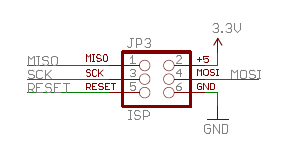
\includegraphics[width=3.5in]{rpi_icsp/icsp-header.png}
    \caption[Arduino ICSP Header]{Pinout of the Arduino Uno and Mega ICSP header}
    \labfig{arduino_icsp_header}
\end{figure}

Note that different microcontrollers may have different implementations of ICSP. Another popular form is the Single
Wire interface. Please refer to your microcontroller's datasheet for specific information.

\section*{Arduino as In-circuit Serial Programmer}

For this example, we will be using an Arduino as an In-circuit Serial Programmer (ISP) to program another Arduino over 
ICSP. The Arduino Foundation provides a sketch in the examples folder of the Arduino IDE to configure an Arduino board 
as an ISP. First, plug in the Arduino Uno to the ICSP header as shown in Figure \ref{fig:arduino_icsp_hookup} and according to Table \ref{tab:arduino_icsp_hookup}. On most boards, there is no reverse-polarity protection, so make sure the 5V and GND wires are plugged in correctly. 

\begin{figure}
    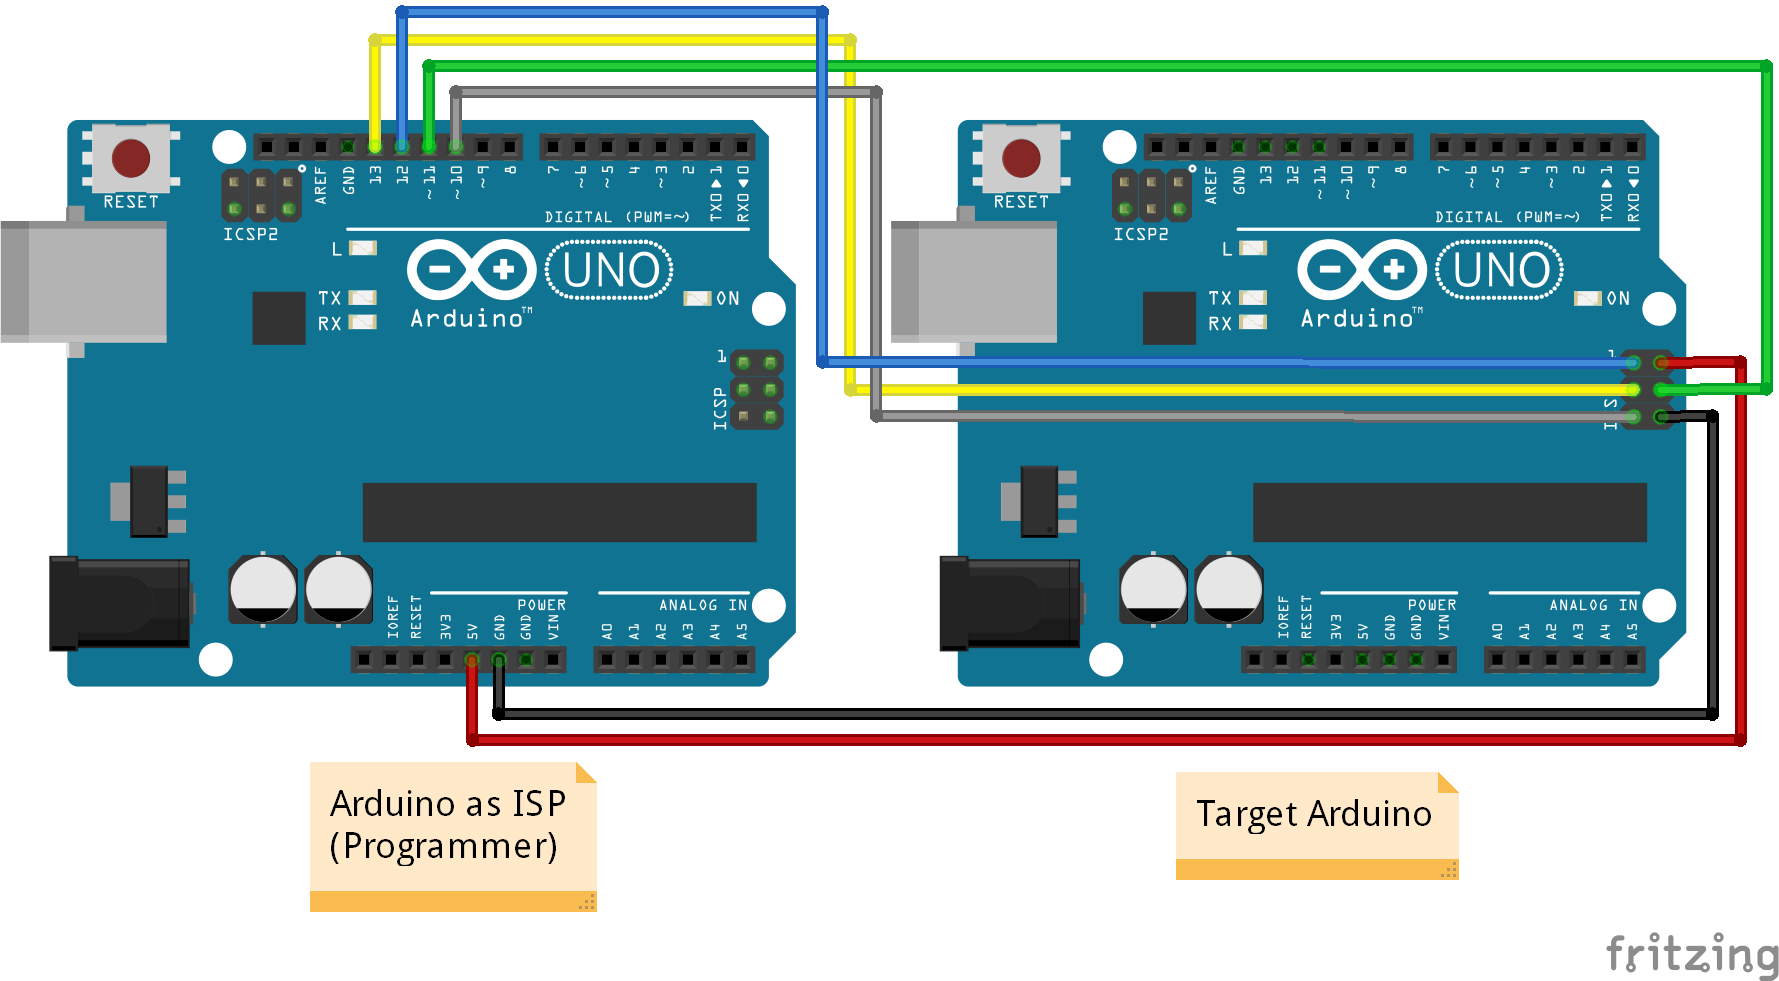
\includegraphics[]{rpi_icsp/Fritzing_ArduinoasISP_AVR_Programmer_bb.png}
    \caption[ArduinoISP Hookup Diagram]{Diagram showing how to hook up an ArduinoISP programmer and Arduino ICSP target.Retrieved from \url{https://learn.sparkfun.com/tutorials/installing-an-arduino-bootloader/hardware-hookup}}
    \labfig{arduino_icsp_hookup}
\end{figure}

\begin{table}[h!]
    \caption[ArduinoISP Hookup Guide]{ArduinoISP hookup table for target and programmer}
    \begin{tabular}{ c | c }
        \toprule
        Programmer & Target \\

        \midrule
        DIO 12  & MISO (Pin 1)  \\
        DIO 13  & SCK (Pin 2)   \\
        DIO 10  & RESET (Pin 3) \\
        5V      & 5V (Pin 4)    \\
        DIO 11  & MOSI (Pin 5)  \\
        GND     & GND (Pin 6)   \\

        \bottomrule
    \end{tabular}
    \labtab{arduino_icsp_hookup}
\end{table}

After wiring up the boards, plug the Arduino Uno into the programming computer. This will apply power to the system and should allow you to program the Uno as you normally would. Then, navigate the ArduinoISP sketch located in the “examples” folder of the Arduino IDE (Figure \ref{fig:arduino_isp_loc}) and upload the sketch to the Arduino Uno.

\begin{figure}
    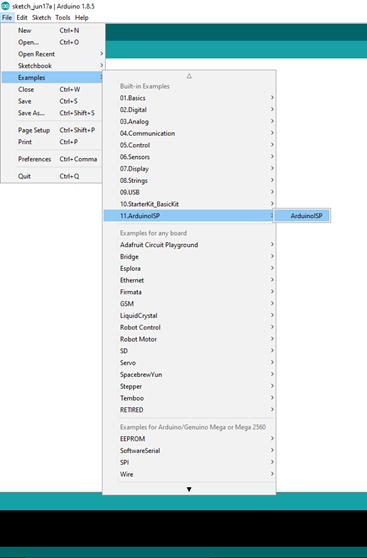
\includegraphics[width=3.5in]{rpi_icsp/ArduinoISP_ss.png}
    \caption[ArduinoISP Example]{Location of ArduinoISP sketch in the Arduino IDE}.
    \labfig{arduino_isp_loc}
\end{figure}

Once the ArduinoISP sketch is uploaded, navigate to a sketch to upload to the target board configuring the compiler to the target board and processor (Figure \ref{fig:arduino_isp_config}). 
Use the same COM port as the Arduino Uno and use the “Upload Using Programmer” option  shown in Figure \ref{fig:arduino_isp_upload}. 
If you get any errors such as “Unable to communicate with device” or “Invalid device signature”, check your wiring and try again.

\begin{figure}
    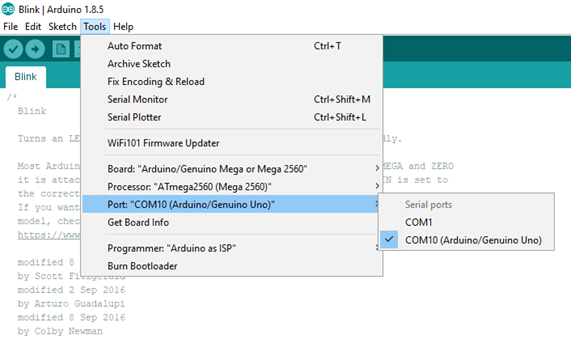
\includegraphics[width=6in]{rpi_icsp/ArduinoISP_config_ss.png}
    \caption[ArduinoISP Config]{Configuring the Arduino IDE to compile for the correct board}.
    \labfig{arduino_isp_config}
\end{figure}

\begin{figure}
    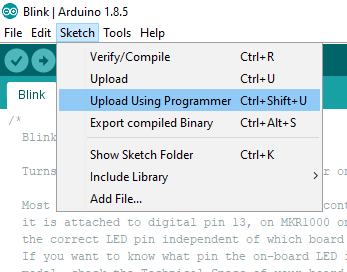
\includegraphics[width=3.5in]{rpi_icsp/ArduinoISP_upload_ss.png}
    \caption[ArduinoISP Upload]{Upload Using Programmer sketch option}.
    \labfig{arduino_isp_upload}
\end{figure}

While this example used the basic Blink example code, this process can be done for any appropriate Arduino sketch onto most Arduino-compatible boards. 
On some embedded devices, a common USB interface may not be accessible and therefore ICSP is the only programming option.

\section*{Using a Raspberry Pi as ISP}

For the graduate portion of this class, we will be using a Raspberry Pi to upload code to the Arduino boards over ICSP. 
The Raspberry Pi uses 3.3V logic levels which are not completely compatible with the 5V logic levels of the Arduino board.
Therefore, it is strongly recommended to use a breadboard to breakout the Raspberry Pi's pins to a logic level converter
and connect it from there to the Arduino's ICSP header. Please refer to Figure \ref{fig:rpi_icsp_bb} for hookup information. 
The pinout for this configuration can be found in the figure, which we will use later with AVRDUDE

    \begin{figure}[h!]
        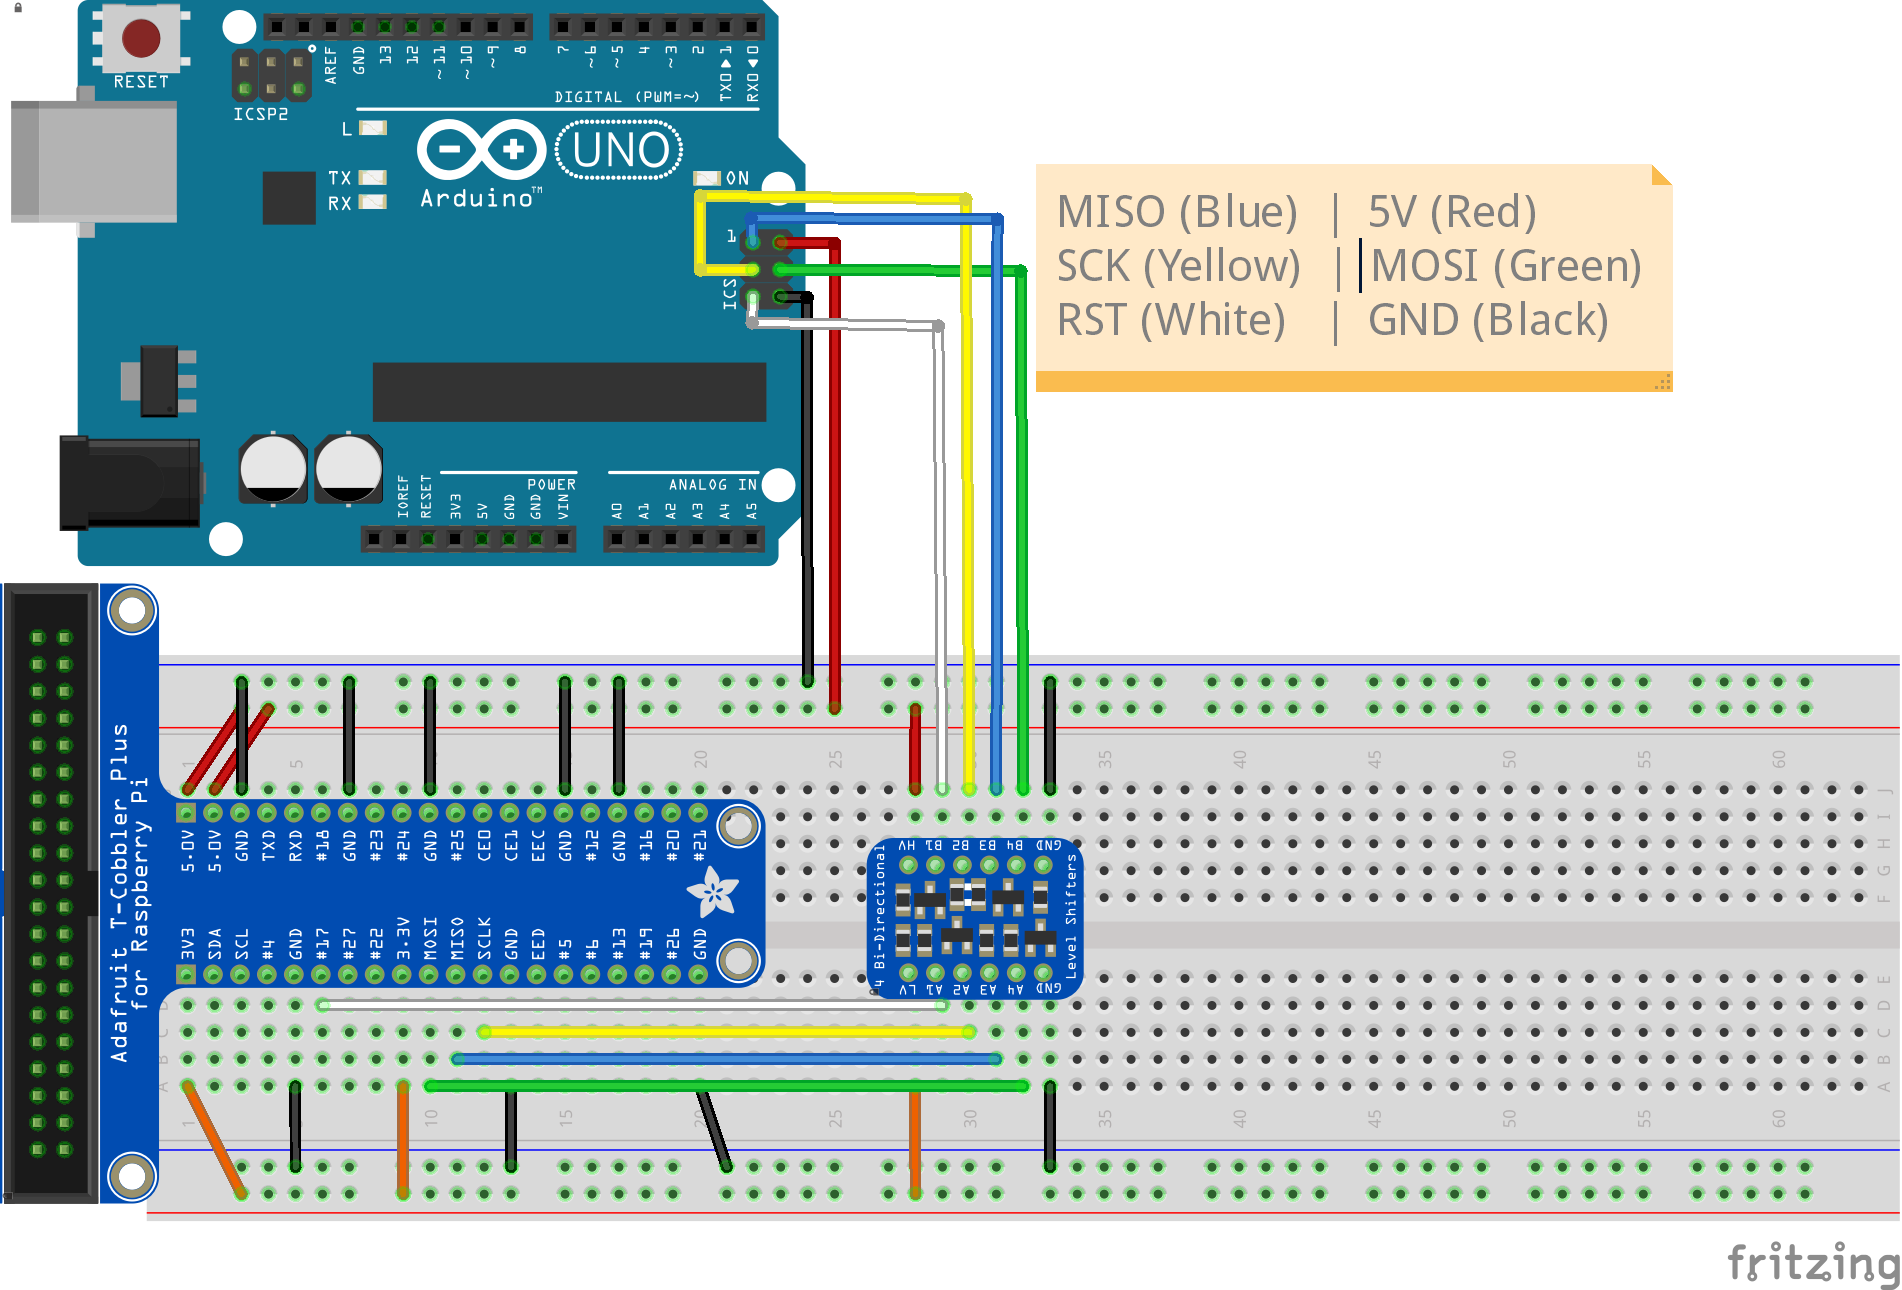
\includegraphics[width=5in]{rpi_icsp/rpi_icsp_bb.png}
        \caption[Raspberry Pi ISP Breadboard]{A wiring diagram of how the Raspberry Pi should be connected to the Arduino ICSP headers through a breadboard and a \href{https://www.adafruit.com/product/757}{logic-level     converter}. 
        Created using Fritzing \url{https://fritzing.org}}.
        \labfig{rpi_icsp_bb}
    \end{figure}

    \begin{table}[h!]
        \caption[RaspberryPi as ISP Hookup Guide]{Raspberry Pi as ISP hookup table for target and programmer}
        \begin{tabular}{ l | c | c }
            \toprule
            Programmer & Logic Level Converter & Target \\
    
            \midrule
            3V3                                 & LV    & NC\footnotemark   \\
            NC\footnotemark[\value{footnote}]   & HV    & 5V                \\
            GPIO 17                             & A1/B1 & RESET             \\
            GPIO 11 (SCLK)                      & A2/B2 & SCK               \\
            GPIO 9 (MISO)                       & A3/B3 & MISO              \\
            GPIO 10 (MOSI)                      & A4/B4 & MOSI              \\
            GND                                 & GND   & GND               \\
    
            \bottomrule
        \end{tabular}
        \labtab{rpi_icsp_hookup}
    \end{table}
    \footnotetext{Not connected}

    \subsection*{Setting up AVRDUDE}
    AVRDUDE is the software package that will upload machine binary to the microcontroller's program storage. 
    The following steps will assume you have already set up the Raspberry Pi with RaspberryPiOS and updated the latest packages. 
    Through this example, we will be operating inside a command terminal through a remote secure login shell, but this process can be repeated inside the command terminal of a headed set up.

    First, in the open terminal execute the following command:

    \begin{lstlisting}[style=kaolstplain,linewidth=1.5\textwidth]
    sudo apt-get install avrdude
    \end{lstlisting}

    This will install AVRDUDE on the Raspberry Pi so we can flash .hex files onto the microcontroller. To verify the installation, execute:

    \begin{lstlisting}[style=kaolstplain,linewidth=1.5\textwidth]
    avrdude -v
    \end{lstlisting}

    If the output is something like:

    \begin{lstlisting}[style=kaolstplain,linewidth=1.5\textwidth]
    avrdude: Version 6.3-20171130
        Copyright (c) 2000-2005 Brian Dean, http://www.bdmicro.com/
        Copyright (c) 2007-2014 Joerg Wunsch

        System wide configuration file is "/etc/avrdude.conf"
        User configuration file is "/home/pi/.avrduderc"
        User configuration file does not exist or is not a regular file, skipping

    avrdude: no programmer has been specified on the command line or the config file
        Specify a programmer using the -c option and try again
    \end{lstlisting}

    Then the installation is good and AVRDUDE has created a user configuration file that we can edit. To begin this process, execute the following commands in the terminal:

    \begin{lstlisting}[style=kaolstplain,linewidth=1.5\textwidth]
    cp /etc/avrdude.conf ~/avrdude_gpio.conf
    \end{lstlisting}

    \begin{lstlisting}[style=kaolstplain,linewidth=1.5\textwidth]
    nano ~/avrdude_gpio.conf
    \end{lstlisting}

    The first command copies the default AVRDUDE configuration file to a new file in the home directory of user. 
    The second command will open this file in the Nano file editor, pulling up a screen like Figure \ref{fig:avrdude_gpio_config_nano}.
    
    \begin{figure}[h!]
        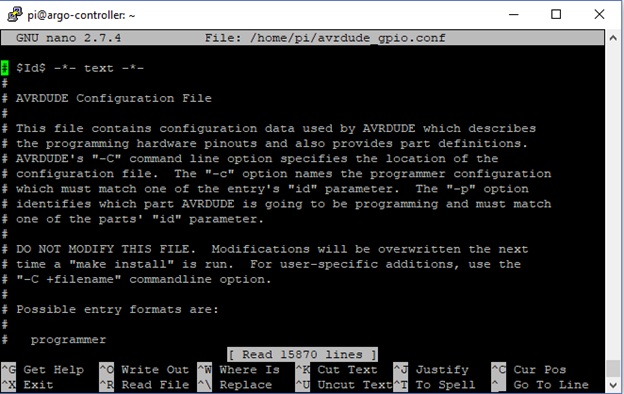
\includegraphics[]{rpi_icsp/avrdude_gpio_conf_nano_ss.png}
        \caption[AVRDUDE GPIO config file open in Nano]{The top of the avrdude\_gpio.conf file in Nano}
        \labfig{avrdude_gpio_config_nano}
    \end{figure}

    Once in the file, press CTRL\+\_, then CTRL\+V to navigate to the bottom of the file. There, paste the following block of code:

    \begin{lstlisting}[style=kaolstplain,linewidth=1.5\textwidth]
    programmer
        id = "gpio_icsp";
        desc = "Use the Linux sysfs interface to bitbang GPIO lines for programming the Arduino;
        type = "linuxgpio";
        reset = 17;
        sck = 11;
        mosi = 10;
        miso = 9;
    ;
    \end{lstlisting}

    This creates an AVRDUDE programmer that uses the GPIO pins specified in Table \ref{tab:rpi_icsp_hookup} to program the Arduino over ICSP. Press CTRL+X then Y then ENTER to save and exit the file; the AVRDUDE programming tool is now configured.

    \subsection*{Preparing a Sketch for ICSP Uploading (Arduino)}

    Once you have a sketch ready for the microcontroller to run, configure the compiler for your board, same as Figure \ref{fig:arduino_isp_config}.
    Select the ``Export compiled Binary'' option in the Arduino IDE (Figure \ref{fig:arduino_ide_export}). 
    This will create two files in the sketch`s directory, both ending with ``.hex'', but one will have ``.with\_bootloader'' in the middle. 
    The file we want to upload is the one without the bootloader, highlighted in Figure \ref{fig:arduino_sketch_folder}. \footnotemark
    
    \footnotetext{This will disable the USB programming bootloader. This will need to be re-flashed with the bootloader if you want to upload code to the microcontroller via USB again.}
    
    \begin{figure}[h!]
        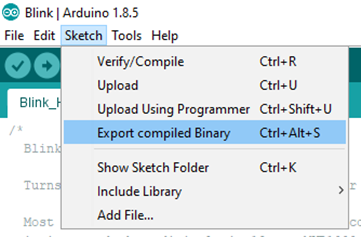
\includegraphics[width=3.5in]{rpi_icsp/arduino_export_binary_ss.png}
        \caption{Arduino IDE ``Export compiled Binary'' option}
        \labfig{arduino_ide_export}
    \end{figure}

    \begin{figure}[h!]
        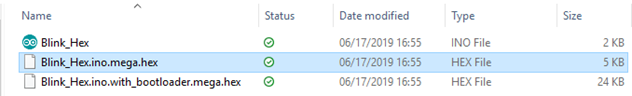
\includegraphics[]{rpi_icsp/arduino_binary_folder_ss.png}
        \caption{The sketch and its compiled binaries in their folder}
        \labfig{arduino_sketch_folder}
    \end{figure}

    \subsection*{Preparing a Sketch for ICSP Uploading (VS Code)}

    This part assumes you have already initialized the Arduino development environment within VS Code.
    In VS Code, open the ``arduino.json'' file in the /.vscode folder of your workspace. Add the following line to the bottom of the file:

    \begin{lstlisting}[style=kaolstplain,linewidth=1.5\textwidth]
    "output": ".arduinobuild"
    \end{lstlisting}

    This will create a new folder in the root directory of the workspace called ``.arduinobuild'' that will hold all of pre-compiled binaries for your Arduino sketch, logs, and other things that are not important right now.
    Inside this folder will be two files: ``[sketch\_name].ino.bin'' and ``[sketch\_name].bootloader.bin''.
    As before, the one we want to upload is the one without the bootloader.\footnotemark[1]

    \subsection*{Programming the Microcontroller}

    Transfer the binary file to the Raspberry Pi using your preferred method of choice.
    This is most easily done over a USB stick or a File Transfer Protocol like Secure Copy.
    Applications like \href{https://winscp.net/eng/download.php}{WinSCP} make this process easy for beginners.
    Place the file in a working destination directory - ideally, a project folder you have already set up beforehand.
    Then, open a terminal on the Raspberry Pi and execute the following command:
    
    \begin{lstlisting}[style=kaolstplain,linewidth=1.5\textwidth]
    sudo avrdude -p [Microcontroller] -C ~/avrdude_gpio.conf -c gpio_icsp -v
    \end{lstlisting}

    Note: the \textbf{[Microcontroller]} in this command needs to be replaced with the name of the microcontroller in use (e.g. ``atmega328p'' for the Arduino Uno or ``atmega2560'' for the Arduino Mega).

    This will verify that the Raspberry Pi can talk to the microcontroller and verifies that the chip is operating nominally.

    If there are any issues, make sure you are executing this command with ``sudo'' and that the configuration file matches with the GPIO pins used in the schematic; check the wiring connections to the Arduino; and check that the file path for ``avrdude\_gpio.conf'' is correct .\footnote{The "\textasciitilde" in the file path only denotes the relative directory you are currently in. If the file is NOT in the same directory that you are executing the command in, you must put the path in lieu of the “\textasciitilde ”.}

    Once you have established communications with the Arduino, execute:

    \begin{lstlisting}[style=kaolstplain,linewidth=1.5\textwidth]
    sudo avrdude -p [Microcontroller] -C ~/avrdude_gpio.conf -c gpio_icsp -v -U flash:w:[filename]:i
    \end{lstlisting}

    Where again \textbf{[Microcontroller]} needs to be replaced with the name of the microcontroller and \textbf{[filename]} needs to be replaced with the path and name of the binary sketch file you copied to the Raspberry Pi.
    The end of a successful write should look something like this:

    \begin{lstlisting}[style=kaolstplain,linewidth=1.5\textwidth]
    avrdude: AVR device initialized and ready to accept instructions

    Reading | ################################################## | 100% 0.00s

    avrdude: Device signature = 0x1e9801 (probably m2560)
    avrdude: safemode: lfuse reads as FF
    avrdude: safemode: hfuse reads as D8
    avrdude: safemode: efuse reads as FD
    avrdude: NOTE: "flash" memory has been specified, an erase cycle will be performed
            To disable this feature, specify the -D option.
    avrdude: erasing chip
    avrdude: reading input file "Blink_Hex.ino.mega.hex"
    avrdude: writing flash (1462 bytes):

    Writing | ################################################## | 100% 0.41s

    avrdude: 1462 bytes of flash written
    avrdude: verifying flash memory against Blink_Hex.ino.mega.hex:
    avrdude: load data flash data from input file Blink_Hex.ino.mega.hex:
    avrdude: input file Blink_Hex.ino.mega.hex contains 1462 bytes
    avrdude: reading on-chip flash data:

    Reading | ################################################## | 100% 0.82s

    avrdude: verifying ...
    avrdude: 1462 bytes of flash verified

    avrdude: safemode: lfuse reads as FF
    avrdude: safemode: hfuse reads as D8
    avrdude: safemode: efuse reads as FD
    avrdude: safemode: Fuses OK (E:FD, H:D8, L:FF)

    avrdude done.  Thank you.
    \end{lstlisting}

    If there is an error (most commonly with a file name) it will likely occur after the first reading block. 
    The -v argument of the command gives error statements in the output so you can error trace and find the problem. 
\pagelayout{margins} % Restore margins

%----------------------------------------------------------------------------------------

\backmatter % Denotes the end of the main document content
\setchapterstyle{plain} % Output plain chapters from this point onwards

%----------------------------------------------------------------------------------------
%	BIBLIOGRAPHY
%----------------------------------------------------------------------------------------

% The bibliography needs to be compiled with biber using your LaTeX editor, or on the command line with 'biber main' from the template directory

% \defbibnote{bibnote}{Here are the references in citation order.\par\bigskip} % Prepend this text to the bibliography
% \printbibliography[heading=bibintoc, title=Bibliography, prenote=bibnote] % Add the bibliography heading to the ToC, set the title of the bibliography and output the bibliography note

%----------------------------------------------------------------------------------------
%	NOMENCLATURE
%----------------------------------------------------------------------------------------

% The nomenclature needs to be compiled on the command line with 'makeindex main.nlo -s nomencl.ist -o main.nls' from the template directory

% \nomenclature{$c$}{Speed of light in a vacuum inertial frame}
% \nomenclature{$h$}{Planck constant}

% \renewcommand{\nomname}{Notation} % Rename the default 'Nomenclature'
% \renewcommand{\nompreamble}{The next list describes several symbols that will be later used within the body of the document.} % Prepend this text to the nomenclature

% \printnomenclature % Output the nomenclature

%----------------------------------------------------------------------------------------
%	GREEK ALPHABET
% 	Originally from https://gitlab.com/jim.hefferon/linear-algebra
%----------------------------------------------------------------------------------------

% \vspace{1cm}

% {\usekomafont{chapter}Greek Letters with Pronunciations} \\[2ex]
% \begin{center}
% 	\newcommand{\pronounced}[1]{\hspace*{.2em}\small\textit{#1}}
% 	\begin{tabular}{l l @{\hspace*{3em}} l l}
% 		\toprule
% 		Character & Name & Character & Name \\ 
% 		\midrule
% 		$\alpha$ & alpha \pronounced{AL-fuh} & $\nu$ & nu \pronounced{NEW} \\
% 		$\beta$ & beta \pronounced{BAY-tuh} & $\xi$, $\Xi$ & xi \pronounced{KSIGH} \\ 
% 		$\gamma$, $\Gamma$ & gamma \pronounced{GAM-muh} & o & omicron \pronounced{OM-uh-CRON} \\
% 		$\delta$, $\Delta$ & delta \pronounced{DEL-tuh} & $\pi$, $\Pi$ & pi \pronounced{PIE} \\
% 		$\epsilon$ & epsilon \pronounced{EP-suh-lon} & $\rho$ & rho \pronounced{ROW} \\
% 		$\zeta$ & zeta \pronounced{ZAY-tuh} & $\sigma$, $\Sigma$ & sigma \pronounced{SIG-muh} \\
% 		$\eta$ & eta \pronounced{AY-tuh} & $\tau$ & tau \pronounced{TOW (as in cow)} \\
% 		$\theta$, $\Theta$ & theta \pronounced{THAY-tuh} & $\upsilon$, $\Upsilon$ & upsilon \pronounced{OOP-suh-LON} \\
% 		$\iota$ & iota \pronounced{eye-OH-tuh} & $\phi$, $\Phi$ & phi \pronounced{FEE, or FI (as in hi)} \\
% 		$\kappa$ & kappa \pronounced{KAP-uh} & $\chi$ & chi \pronounced{KI (as in hi)} \\
% 		$\lambda$, $\Lambda$ & lambda \pronounced{LAM-duh} & $\psi$, $\Psi$ & psi \pronounced{SIGH, or PSIGH} \\
% 		$\mu$ & mu \pronounced{MEW} & $\omega$, $\Omega$ & omega \pronounced{oh-MAY-guh} \\
% 		\bottomrule
% 	\end{tabular} \\[1.5ex]
% 	Capitals shown are the ones that differ from Roman capitals.
% \end{center}

%----------------------------------------------------------------------------------------
%	GLOSSARY
%----------------------------------------------------------------------------------------

% The glossary needs to be compiled on the command line with 'makeglossaries main' from the template directory

% \setglossarystyle{listgroup} % Set the style of the glossary (see https://en.wikibooks.org/wiki/LaTeX/Glossary for a reference)
% \printglossary[title=Special Terms, toctitle=List of Terms] % Output the glossary, 'title' is the chapter heading for the glossary, toctitle is the table of contents heading

%----------------------------------------------------------------------------------------
%	INDEX
%----------------------------------------------------------------------------------------

% The index needs to be compiled on the command line with 'makeindex main' from the template directory

% \printindex % Output the index

%----------------------------------------------------------------------------------------
%	BACK COVER
%----------------------------------------------------------------------------------------

% If you have a PDF/image file that you want to use as a back cover, uncomment the following lines

%\clearpage
%\thispagestyle{empty}
%\null%
%\clearpage
%\includepdf{cover-back.pdf}

%----------------------------------------------------------------------------------------

\end{document}
